%%%%%%%%%%%%%%%%%%%%%%%%%%%%%%%%%%%%%%%%
% datoteka diploma-vzorec.tex
%
% vzorčna datoteka za pisanje diplomskega dela v formatu LaTeX
% na UL Fakulteti za računalništvo in informatiko
%
% vkup spravil Gašper Fijavž, december 2010
% 
%
%
% verzija 12. februar 2014 (besedilo teme, seznam kratic, popravki Gašper Fijavž)
% verzija 10. marec 2014 (redakcijski popravki Zoran Bosnić)
% verzija 11. marec 2014 (redakcijski popravki Gašper Fijavž)
% verzija 15. april 2014 (pdf/a 1b compliance, not really - just claiming, Damjan Cvetan, Gašper Fijavž)
% verzija 23. april 2014 (privzeto cc licenca)
% verzija 16. september 2014 (odmiki strain od roba)
% verzija 28. oktober 2014 (odstranil vpisno številko)
% verija 5. februar 2015 (Literatura v kazalu, online literatura)
% verzija 25. september 2015 (angl. naslov v izjavi o avtorstvu)
% verzija 26. februar 2016 (UL izjava o avtorstvu)
% verzija 16. april 2016 (odstranjena izjava o avtorstvu)
% verzija 5. junij 2016 (Franc Solina dodal vrstice, ki jih je označil s svojim imenom)


\documentclass[a4paper, 12pt]{book}
%\documentclass[a4paper, 12pt, draft]{book}  Nalogo preverite tudi z opcijo draft, ki vam bo pokazala, katere vrstice so predolge!



\usepackage[utf8x]{inputenc}   % omogoča uporabo slovenskih črk kodiranih v formatu UTF-8
\usepackage[slovene,english]{babel}    % naloži, med drugim, slovenske delilne vzorce
\usepackage[pdftex]{graphicx}  % omogoča vlaganje slik različnih formatov
\usepackage{fancyhdr}          % poskrbi, na primer, za glave stranif
\usepackage{amssymb}           % dodatni simboli
\usepackage{amsmath}           % eqref, npr.
%\usepackage{hyperxmp}
\usepackage[hyphens]{url}  % dodal Solina
\usepackage{comment}       % dodal Solina

\usepackage[pdftex, colorlinks=true,
						citecolor=black, filecolor=black, 
						linkcolor=black, urlcolor=black,
						pagebackref=false, 
						pdfproducer={LaTeX}, pdfcreator={LaTeX}, hidelinks]{hyperref}

\usepackage{color}       % dodal Solina
\usepackage{soul}       % dodal Solina

%%%%%%%%%%%%%%%%%%%%%%%%%%%%%%%%%%%%%%%%
%	DIPLOMA INFO
%%%%%%%%%%%%%%%%%%%%%%%%%%%%%%%%%%%%%%%%
\newcommand{\ttitle}{Elektronsko naročanje v restavraciji}
\newcommand{\ttitleEn}{Electronic ordering in a restaurant}
\newcommand{\tsubject}{\ttitle}
\newcommand{\tsubjectEn}{\ttitleEn}
\newcommand{\tauthor}{Luka Horvat}
\newcommand{\tkeywords}{spletna aplikacija, elektronsko naročanje, restavracija, Vue, JavaScript}
\newcommand{\tkeywordsEn}{web application, electronic ordering, restaurant, Vue, JavaScript}

%%%%%%%%%%%%%%%%%%%%%%%%%%%%%%%%%%%%%%%%
%	HYPERREF SETUP
%%%%%%%%%%%%%%%%%%%%%%%%%%%%%%%%%%%%%%%%
\hypersetup{pdftitle={\ttitle}}
\hypersetup{pdfsubject=\ttitleEn}
\hypersetup{pdfauthor={\tauthor, matjaz.kralj@fri.uni-lj.si}}
\hypersetup{pdfkeywords=\tkeywordsEn}

%%%%%%%%%%%%%%%%%%%%%%%%%%%%%%%%%%%%%%%%
% znaki za copyright stran
%%%%%%%%%%%%%%%%%%%%%%%%%%%%%%%%%%%%%%%%  

\newcommand{\CcImageCc}[1]{%
	
\includegraphics[scale=#1]{cc_cc_30.pdf}%
}
\newcommand{\CcImageBy}[1]{%
	
\includegraphics[scale=#1]{cc_by_30.pdf}%
}
\newcommand{\CcImageSa}[1]{%
	
\includegraphics[scale=#1]{cc_sa_30.pdf}%
}

 


%%%%%%%%%%%%%%%%%%%%%%%%%%%%%%%%%%%%%%%%
% postavitev strani
%%%%%%%%%%%%%%%%%%%%%%%%%%%%%%%%%%%%%%%%  

\addtolength{\marginparwidth}{-20pt} % robovi za tisk
\addtolength{\oddsidemargin}{40pt}
\addtolength{\evensidemargin}{-40pt}

\renewcommand{\baselinestretch}{1.3} % ustrezen razmik med vrsticami
\setlength{\headheight}{15pt}        % potreben prostor na vrhu
\renewcommand{\chaptermark}[1]%
{\markboth{\MakeUppercase{\thechapter.\ #1}}{}} \renewcommand{\sectionmark}[1]%
{\markright{\MakeUppercase{\thesection.\ #1}}} \renewcommand{\headrulewidth}{0.5pt} \renewcommand{\footrulewidth}{0pt}
\fancyhf{}
\fancyhead[LE,RO]{\sl \thepage} 
%\fancyhead[LO]{\sl \rightmark} \fancyhead[RE]{\sl \leftmark}
\fancyhead[RE]{\sc \tauthor}              % dodal Solina
\fancyhead[LO]{\sc Diplomska naloga}     % dodal Solina


\newcommand{\BibTeX}{{\sc Bib}\TeX}

%%%%%%%%%%%%%%%%%%%%%%%%%%%%%%%%%%%%%%%%
% naslovi
%%%%%%%%%%%%%%%%%%%%%%%%%%%%%%%%%%%%%%%%  

\newcommand{\autfont}{\Large}
\newcommand{\titfont}{\LARGE\bf}
\newcommand{\clearemptydoublepage}{\newpage{\pagestyle{empty}\cleardoublepage}}
\setcounter{tocdepth}{2}	      % globina kazala

%%%%%%%%%%%%%%%%%%%%%%%%%%%%%%%%%%%%%%%%
% konstrukti
%%%%%%%%%%%%%%%%%%%%%%%%%%%%%%%%%%%%%%%%  
\newtheorem{izrek}{Izrek}[chapter]
\newtheorem{trditev}{Trditev}[izrek]
\newenvironment{dokaz}{\emph{Dokaz.}\ }{\hspace{\fill}{$\Box$}}

%%%%%%%%%%%%%%%%%%%%%%%%%%%%%%%%%%%%%%%%%%%%%%%%%%%%%%%%%%%%%%%%%%%%%%%%%%%%%%%
%% PDF-A
%%%%%%%%%%%%%%%%%%%%%%%%%%%%%%%%%%%%%%%%%%%%%%%%%%%%%%%%%%%%%%%%%%%%%%%%%%%%%%%


%%%%%%%%%%%%%%%%%%%%%%%%%%%%%%%%%%%%%%%% 
% define medatata
%%%%%%%%%%%%%%%%%%%%%%%%%%%%%%%%%%%%%%%% 
\def\Title{\ttitle}
\def\Author{\tauthor, lh8069@fri.uni-lj.si}
\def\Subject{\ttitleEn}
\def\Keywords{\tkeywordsEn}

%%%%%%%%%%%%%%%%%%%%%%%%%%%%%%%%%%%%%%%% 
% \convertDate converts D:20080419103507+02'00' to 2008-04-19T10:35:07+02:00
%%%%%%%%%%%%%%%%%%%%%%%%%%%%%%%%%%%%%%%% 
\def\convertDate{%
    \getYear
}

{\catcode`\D=12
 \gdef\getYear D:#1#2#3#4{\edef\xYear{#1#2#3#4}\getMonth}
}
\def\getMonth#1#2{\edef\xMonth{#1#2}\getDay}
\def\getDay#1#2{\edef\xDay{#1#2}\getHour}
\def\getHour#1#2{\edef\xHour{#1#2}\getMin}
\def\getMin#1#2{\edef\xMin{#1#2}\getSec}
\def\getSec#1#2{\edef\xSec{#1#2}\getTZh}
\def\getTZh +#1#2{\edef\xTZh{#1#2}\getTZm}
\def\getTZm '#1#2'{%
    \edef\xTZm{#1#2}%
    \edef\convDate{\xYear-\xMonth-\xDay T\xHour:\xMin:\xSec+\xTZh:\xTZm}%
}

\expandafter\convertDate\pdfcreationdate 

%%%%%%%%%%%%%%%%%%%%%%%%%%%%%%%%%%%%%%%%
% get pdftex version string
%%%%%%%%%%%%%%%%%%%%%%%%%%%%%%%%%%%%%%%% 
\newcount\countA
\countA=\pdftexversion
\advance \countA by -100
\def\pdftexVersionStr{pdfTeX-1.\the\countA.\pdftexrevision}


%%%%%%%%%%%%%%%%%%%%%%%%%%%%%%%%%%%%%%%%
% XMP data
%%%%%%%%%%%%%%%%%%%%%%%%%%%%%%%%%%%%%%%%  
\usepackage{xmpincl}
\includexmp{pdfa-1b}

%%%%%%%%%%%%%%%%%%%%%%%%%%%%%%%%%%%%%%%%
% pdfInfo
%%%%%%%%%%%%%%%%%%%%%%%%%%%%%%%%%%%%%%%%  
\pdfinfo{%
    /Title    (\ttitle)
    /Author   (\tauthor, damjan@cvetan.si)
    /Subject  (\ttitleEn)
    /Keywords (\tkeywordsEn)
    /ModDate  (\pdfcreationdate)
    /Trapped  /False
}


%%%%%%%%%%%%%%%%%%%%%%%%%%%%%%%%%%%%%%%%%%%%%%%%%%%%%%%%%%%%%%%%%%%%%%%%%%%%%%%
%%%%%%%%%%%%%%%%%%%%%%%%%%%%%%%%%%%%%%%%%%%%%%%%%%%%%%%%%%%%%%%%%%%%%%%%%%%%%%%

\begin{document}
\selectlanguage{slovene}
\frontmatter
\setcounter{page}{1} %
\renewcommand{\thepage}{}       % preprecimo težave s številkami strani v kazalu
\newcommand{\sn}[1]{"`#1"'}                    % dodal Solina (slovenski narekovaji)

%%%%%%%%%%%%%%%%%%%%%%%%%%%%%%%%%%%%%%%%
%naslovnica
 \thispagestyle{empty}%
   \begin{center}
    {\large\sc Univerza v Ljubljani\\%
      Fakulteta za računalništvo in informatiko}%
    \vskip 10em%
    {\autfont \tauthor\par}%
    {\titfont \ttitle \par}%
    {\vskip 3em \textsc{DIPLOMSKO DELO\\[5mm]         % dodal Solina za ostale študijske programe
%    VISOKOŠOLSKI STROKOVNI ŠTUDIJSKI PROGRAM\\ PRVE STOPNJE\\ RAČUNALNIŠTVO IN INFORMATIKA}\par}%
    VISOKOŠOLSKI STROKOVNI ŠTUDIJSKI PROGRAM \\ PRVE STOPNJE\\ RAČUNALNIŠTVO IN INFORMATIKA}\par}%
%    INTERDISCIPLINARNI UNIVERZITETNI\\ ŠTUDIJSKI PROGRAM PRVE STOPNJE\\ RAČUNALNIŠTVO IN MATEMATIKA}\par}%
%    INTERDISCIPLINARNI UNIVERZITETNI\\ ŠTUDIJSKI PROGRAM PRVE STOPNJE\\ UPRAVNA INFORMATIKA}\par}%
%    INTERDISCIPLINARNI UNIVERZITETNI\\ ŠTUDIJSKI PROGRAM PRVE STOPNJE\\ MULTIMEDIJA}\par}%
    \vfill\null%
    {\large \textsc{Mentorica}: doc. dr. Mira Trebar\par}%
   {\large \textsc{Somentor}: as. dr. David Jelenc \par}%
    {\vskip 2em \large Ljubljana, 2022 \par}%
\end{center}
% prazna stran
%\clearemptydoublepage      % dodal Solina (izjava o licencah itd. se izpiše na hrbtni strani naslovnice)

%%%%%%%%%%%%%%%%%%%%%%%%%%%%%%%%%%%%%%%%
%copyright stran
\vspace*{5cm}
{\small \noindent
To delo je ponujeno pod licenco \textit{Creative Commons Priznanje avtorstva-Deljenje pod enakimi pogoji 2.5 Slovenija} (ali novej\v so razli\v cico).
To pomeni, da se tako besedilo, slike, grafi in druge sestavine dela kot tudi rezultati diplomskega dela lahko prosto distribuirajo,
reproducirajo, uporabljajo, priobčujejo javnosti in predelujejo, pod pogojem, da se jasno in vidno navede avtorja in naslov tega
dela in da se v primeru spremembe, preoblikovanja ali uporabe tega dela v svojem delu, lahko distribuira predelava le pod
licenco, ki je enaka tej.
Podrobnosti licence so dostopne na spletni strani \href{http://creativecommons.si}{creativecommons.si} ali na Inštitutu za
intelektualno lastnino, Streliška 1, 1000 Ljubljana.

\vspace*{1cm}
\begin{center}% 0.66 / 0.89 = 0.741573033707865
\CcImageCc{0.741573033707865}\hspace*{1ex}\CcImageBy{1}\hspace*{1ex}\CcImageSa{1}%
\end{center}
}

\vspace*{1cm}
{\small \noindent
Izvorna koda diplomskega dela, njeni rezultati in v ta namen razvita programska oprema je ponujena pod licenco GNU General Public License,
različica 3 (ali novejša). To pomeni, da se lahko prosto distribuira in/ali predeluje pod njenimi pogoji.
Podrobnosti licence so dostopne na spletni strani \url{http://www.gnu.org/licenses/}.
}

\vfill
\begin{center} 
\ \\ \vfill
{\em
Besedilo je oblikovano z urejevalnikom besedil \LaTeX.}
\end{center}
% prazna stran
\clearemptydoublepage

%%%%%%%%%%%%%%%%%%%%%%%%%%%%%%%%%%%%%%%%
% stran 3 med uvodnimi listi
\thispagestyle{empty}
\
\vfill

\bigskip
\noindent\textbf{Kandidat:} Luka Horvat\\
\noindent\textbf{Naslov:} Elektronsko naročanje v restavraciji\\
% vstavite ustrezen naziv študijskega programa!
\noindent\textbf{Vrsta naloge:} Diplomska naloga na visokošolskem strokovnem programu prve stopnje Računalništvo in informatika \\
% izberite pravi habilitacijski naziv mentorja!
\noindent\textbf{Mentor:} doc. dr. Mira Trebar\\
\noindent\textbf{Somentor:} as. dr. David Jelenc

\bigskip
\noindent\textbf{Opis:}\\
Kandidat naj v diplomskem delu analizira postopek obdelave naročil v restavraciji. Zasnuje naj spletno aplikacijo, ki omogoča gostom pregled ponudbe in izvedbo naročil. Osebje naj ima možnost urejanja, spremljanje in izvedbo ter zaključitev postopka z izdajo računa v stvarnem času. Za implementiran model odjemalec-strežnik naj predstavi enostaven primer uporabe vmesnikov za gosta, natakarja in kuharja.

\bigskip
\noindent\textbf{Title:} Electronic ordering in a restaurant

\bigskip
\noindent\textbf{Description:}\\
The candidate is instructed to analyze the process of ordering food and beverages in a restaurant. A web application is to be developed that supports said process and allows guests to review the offer and order items. Restaurant staff should be able to oversee, modify, confirm, and complete orders by issuing an invoice, all in real-time. The candidate is to present example interface for the roles of guest, the waiter and the chef.

\vfill



\vspace{2cm}

% prazna stran
\clearemptydoublepage

% zahvala
\thispagestyle{empty}\mbox{}\vfill\null\it%
\noindent
Zahvaljujem se mentorici doc. dr. Miri Trebar in somentorju as. dr. Davidu Jelencu za vso pomoč in nasvete.
Zahvaljujem se tudi ožji družini in punci za podporo.
\rm\normalfont

% prazna stran
\clearemptydoublepage

%%%%%%%%%%%%%%%%%%%%%%%%%%%%%%%%%%%%%%%%
% posvetilo, če sama zahvala ne zadošča :-)
%\thispagestyle{empty}\mbox{}{\vskip0.20\textheight}\mbox{}\hfill\begin{minipage}{0.55\textwidth}%
%Svoji dragi Alenčici.
%\normalfont\end{minipage}

% prazna stran
\clearemptydoublepage


%%%%%%%%%%%%%%%%%%%%%%%%%%%%%%%%%%%%%%%%
% kazalo
\pagestyle{empty}
\def\thepage{}% preprecimo tezave s stevilkami strani v kazalu
\tableofcontents{}

% prazna stran
\clearemptydoublepage

%%%%%%%%%%%%%%%%%%%%%%%%%%%%%%%%%%%%%%%%
% seznam kratic

\chapter*{Seznam uporabljenih kratic}  % spremenil Solina, da predolge vrstice ne gredo preko desnega roba

\begin{comment}
\begin{tabular}{l|l|l}
  {\bf kratica} & {\bf angleško} & {\bf slovensko} \\ \hline
  % after \\: \hline or \cline{col1-col2} \cline{col3-col4} ...
  {\bf SPA} & single page application & aplikacija na eni strani \\
  {\bf SQL} & structured query language & strukturirani povpraševalni jezik za delo s podatkovnimi bazami  \\
  {\bf SVM} & support vector machine & metoda podpornih vektorjev \\
  {\bf SVM}   & support vector machine              & metoda podpornih vektorjev \\
  \dots & \dots & \dots \\
\end{tabular}
\end{comment}

\noindent\begin{tabular}{p{0.1\textwidth}|p{.4\textwidth}|p{.4\textwidth}}    % po potrebi razširi prvo kolono tabele na račun drugih dveh!
  {\bf kratica} & {\bf angleško}                             & {\bf slovensko} \\ \hline
  {\bf API}   &  application programming interface              & programski vmesnik\\
  {\bf CLI}   & command-line interface              & ukazno-vrstični vmesnik \\
  {\bf DBMS}   &  database management system              & sistem za upravljanje podatkovne baze \\
  {\bf ENUM}   & enumerated type              & naštevni tip \\
  {\bf HTTP}   &  hypertext transfer protocol               &  protokol svetovnega spleta \\
  {\bf JSON}   &  JavaScript object notation               &  objektna notacija za JavaScript \\
  {\bf QR}   &  quick response              & hiter odziv\\
  {\bf REST}   & representational state transfer              & reprezentativni prenos stanja \\
  {\bf SPA}      & single page application               &  enostranska aplikacija \\	
  {\bf SQL} & structured query language & poizvedovalni jezik SQL  \\
  {\bf URI}   &  uniform resource identifier              & enotni identifikator vira \\
  {\bf XML}   &  extensible markup language              & razširljiv označevalni jezik \\

%  \dots & \dots & \dots \\
\end{tabular}


% prazna stran
\clearemptydoublepage

%%%%%%%%%%%%%%%%%%%%%%%%%%%%%%%%%%%%%%%%
% povzetek
\addcontentsline{toc}{chapter}{Povzetek}
\chapter*{Povzetek}

\noindent\textbf{Naslov:} \ttitle
\bigskip

\noindent\textbf{Avtor:} \tauthor
\bigskip


%\noindent\textbf{Povzetek:} 
\noindent 
Diplomsko delo zajema analizo, načrtovanje in razvoj spletne aplikacije, ki omogoča elektronsko naročanje hrane in pijače v restavracijah. Namen aplikacije je olajšati delo natakarjem in nuditi kakovostnejšo postrežbo gostom. Ključne funkcionalnosti so oddajanje naročil za gosta ter nadzor in upravljanje naročil za natakarja in kuharja. Omogočeno je naročanje preko aplikacije ali z neposrednim stikom z natakarjem. Aplikacija je zasnovana kot visokonivojska arhitektura (model odjemalec-strežnik), ki jo sestavljajo aplikacija, strežnik in podatkovna baza. Za razvoj aplikacije so uporabljeni ogrodje Vue in programski jeziki JavaScript, Python ter MySQL za podatkovno bazo.
\bigskip

\noindent\textbf{Ključne besede:} \tkeywords.
% prazna stran
\clearemptydoublepage

%%%%%%%%%%%%%%%%%%%%%%%%%%%%%%%%%%%%%%%%
% abstract
\selectlanguage{english}
\addcontentsline{toc}{chapter}{Abstract}
\chapter*{Abstract}

\noindent\textbf{Title:} \ttitleEn
\bigskip

\noindent\textbf{Author:} \tauthor
\bigskip

%\noindent\textbf{Abstract:} 
\noindent The diploma thesis covers the analysis, design, and development of a web application for restaurant's electronic ordering of food and beverages. The purpose of the application is to facilitate the waiter's work and provide better quality service to guests. The key functionalities are placing orders by the guest and the control and management of orders by the waiter and the chef. It is possible to order via this application or directly contact the waiter. The application is designed as a high-level architecture (client-server model), consisting of the application, server, and database. The Vue framework and JavaScript, Python, and MySQL database languages are used in the development of the application.
\bigskip

\noindent\textbf{Keywords:} \tkeywordsEn.
\selectlanguage{slovene}
% prazna stran
\clearemptydoublepage

%%%%%%%%%%%%%%%%%%%%%%%%%%%%%%%%%%%%%%%%
\mainmatter
\setcounter{page}{1}
\pagestyle{fancy}
 
\chapter{Uvod}
Slovenija velja za državo z veliko restavracijami, vendar le redke med njimi uporabljajo napredne sisteme naročanja kot npr. ena izmed večjih verig s hitro prehrano, McDonald's. V Sloveniji so obstajali projekti s podobnimi idejami, vendar do sedaj nismo zasledili takšnih rešitev. Problematiko smo vzeli kot motivacijo ter si zadali cilj, da izdelamo aplikacijo kot pripomoček za optimizacijo dela natakarjev. Ker ustrezne rešitve za ta problem nismo zaznali, nam pa se je zdelo, da jo lahko realiziramo, smo se odločili v diplomski nalogi razviti izvedbo elektronskega naročanja hrane in pijače.

Zamislili smo si sistem za oddajanje naročil v restavracijah, ki ne bi nadomestil ljudi v strežbi, temveč bi služil kot pregledovalnik ponudbe z možnostjo naročanja hrane in pijače. Aplikacija bi bila na tablicah, ki bi bile nameščene na vsaki mizi restavracije. Stranka bi bila tista, ki bi se odločala, ali želi pri naročanju uporabiti stik z osebo v strežbi ali bi naročila z uporabo aplikacije na tablici. Delovanje bi bilo sledeče: stranka oziroma gost odda naročilo, natakar in kuhar ga preverita, potrdita in pripravita. Posledično bi bile stranke, ki veljajo za zahtevnejše in bolj neučakane na vseh področjih, hitreje in kakovostneje postrežene. 

Diplomsko delo je razdeljeno na dva dela. V prvem delu je opisan postopek načrtovanja in razvoj aplikacije. To pomeni opis komponent, ki sestavljajo samo arhitekturo aplikacije, kako se med seboj povezujejo in sestavljajo delujoč sistem. V drugem delu je predstavljeno delovanje aplikacije, najprej podrobneje, nato na podlagi primera. V nadaljevanju so navedene tudi omejitve naše rešitve in mogoče izboljšave. Na koncu so dodane še sklepne ugotovitve. 

\chapter{Načrtovanje in razvoj aplikacije}

Načrtovanje aplikacije je potekalo v treh delih in je vključevalo opis zahtev oziroma izdelavo diagrama primerov uporabe, razvoj arhitekture in izbiro tehnologij. Predlagana rešitev je bila v nadaljevanju osnova za izdelavo dveh spletnih aplikacij. Ena aplikacija je namenjena gostom, druga pa natakarjem in kuharjem. Restavracija ima lahko več miz, vendar je za eno mizo lahko hkrati odprto eno naročilo. To pomeni, da morajo vsi gosti za mizo naročati skupaj. Slika~\ref{FunkVloge} prikazuje primere uporabe za izvedbo celotnega naročila. 

Gost lahko odda, spremeni ali zaključi naročilo. Funkcionalnost za gosta so: dodajanje artiklov v naročilo in brisanje teh iz njega, oddajanje, urejanje in pregledovanje naročila, spremljanje statusa naročila in zahtevanje računa. 

Natakar lahko potrdi, uredi ali zaključi naročilo. V restavraciji je lahko več natakarjev, ki svoja naročila vodijo preko ločene prijave. Funkcionalnosti za natakarja so: potrjevanje, urejanje in pregledovanje naročila, spremljanje statusa in statistike naročil in možnost tiskanja računa za določeno naročilo. Kuhar lahko potrdi ali zavrne naročilo ter obvesti natakarja o zaključku priprave jedi za določeno naročilo. Restavracija lahko ima več kuharjev, vendar vsi uporabljajo aplikacijo preko iste prijave. Omejitev je v podatkovnem modelu. Funkcionalnosti za kuharja so: pregledovanje, potrjevanje in zavračanje naročila, obveščanje natakarja o zaključku priprave jedi ter spremljanje statistike naročil. 

\begin{figure}[!htb]
\centering
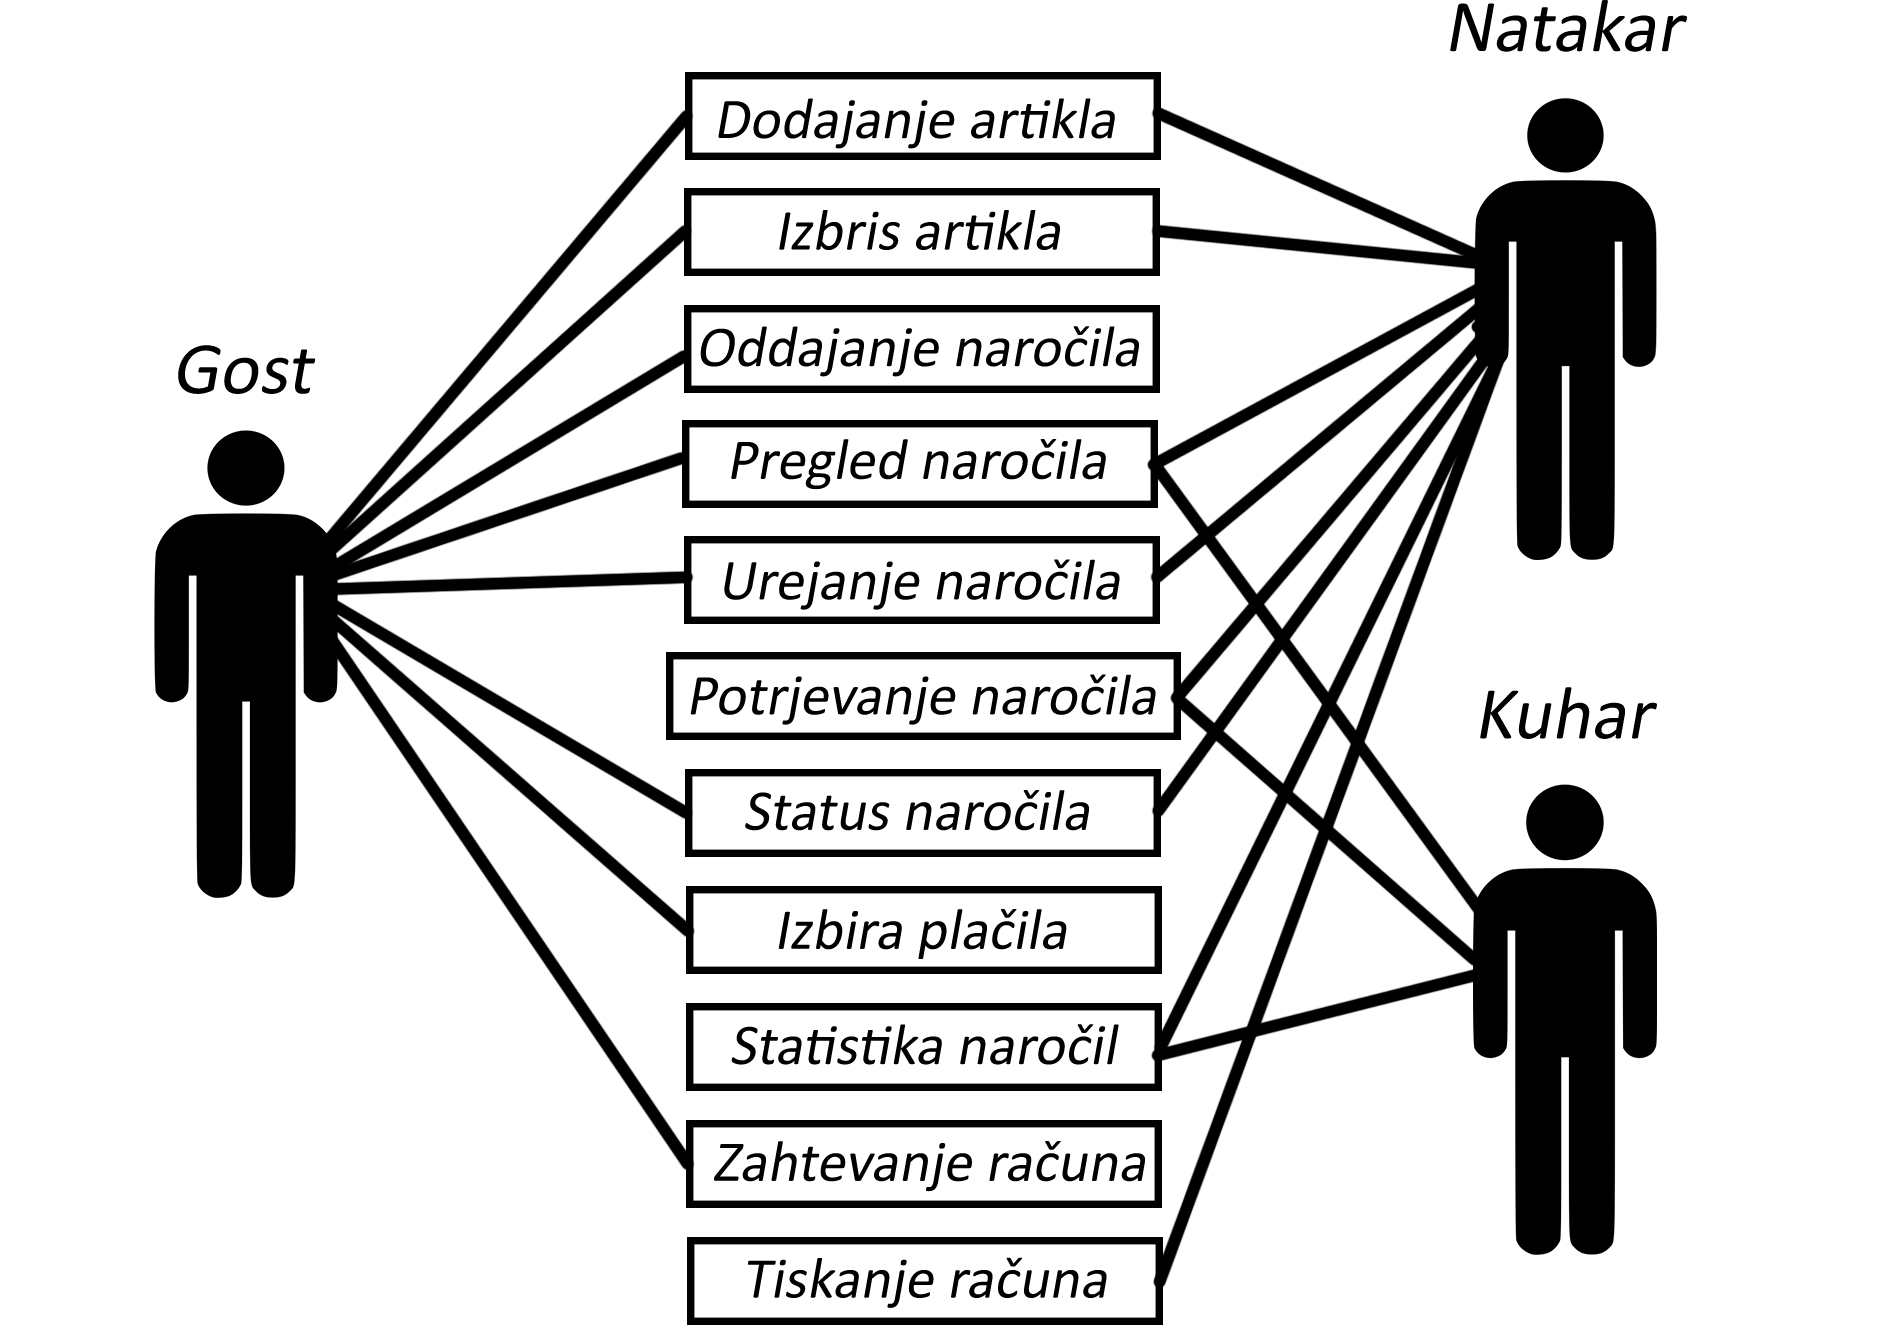
\includegraphics[width=10.8cm]{Skica2.png}
\caption{Diagram primerov uporabe spletnega naročanja}
\label{FunkVloge}
\end{figure}

Uporabili smo trenutno najbolj razširjeno arhitekturo, ki jo sestavljajo podatkovna baza, strežnik in aplikacija oziroma odjemalec. To je koncept, ki ga je mogoče prilagajati predvsem z uporabniškega vidika. Slika~\ref{StrukApk} prikazuje arhitekturno rešitev aplikacije \cite{TRINIVO}.
Podatkovna baza je namenjena shranjevanju vseh podatkov za posamezno restavracijo. Strežnik implementira vmesnik RESTful, ki odjemalcu oziroma aplikaciji posreduje podatke iz podatkovne baze. 

\begin{figure}[!htb]
\centering
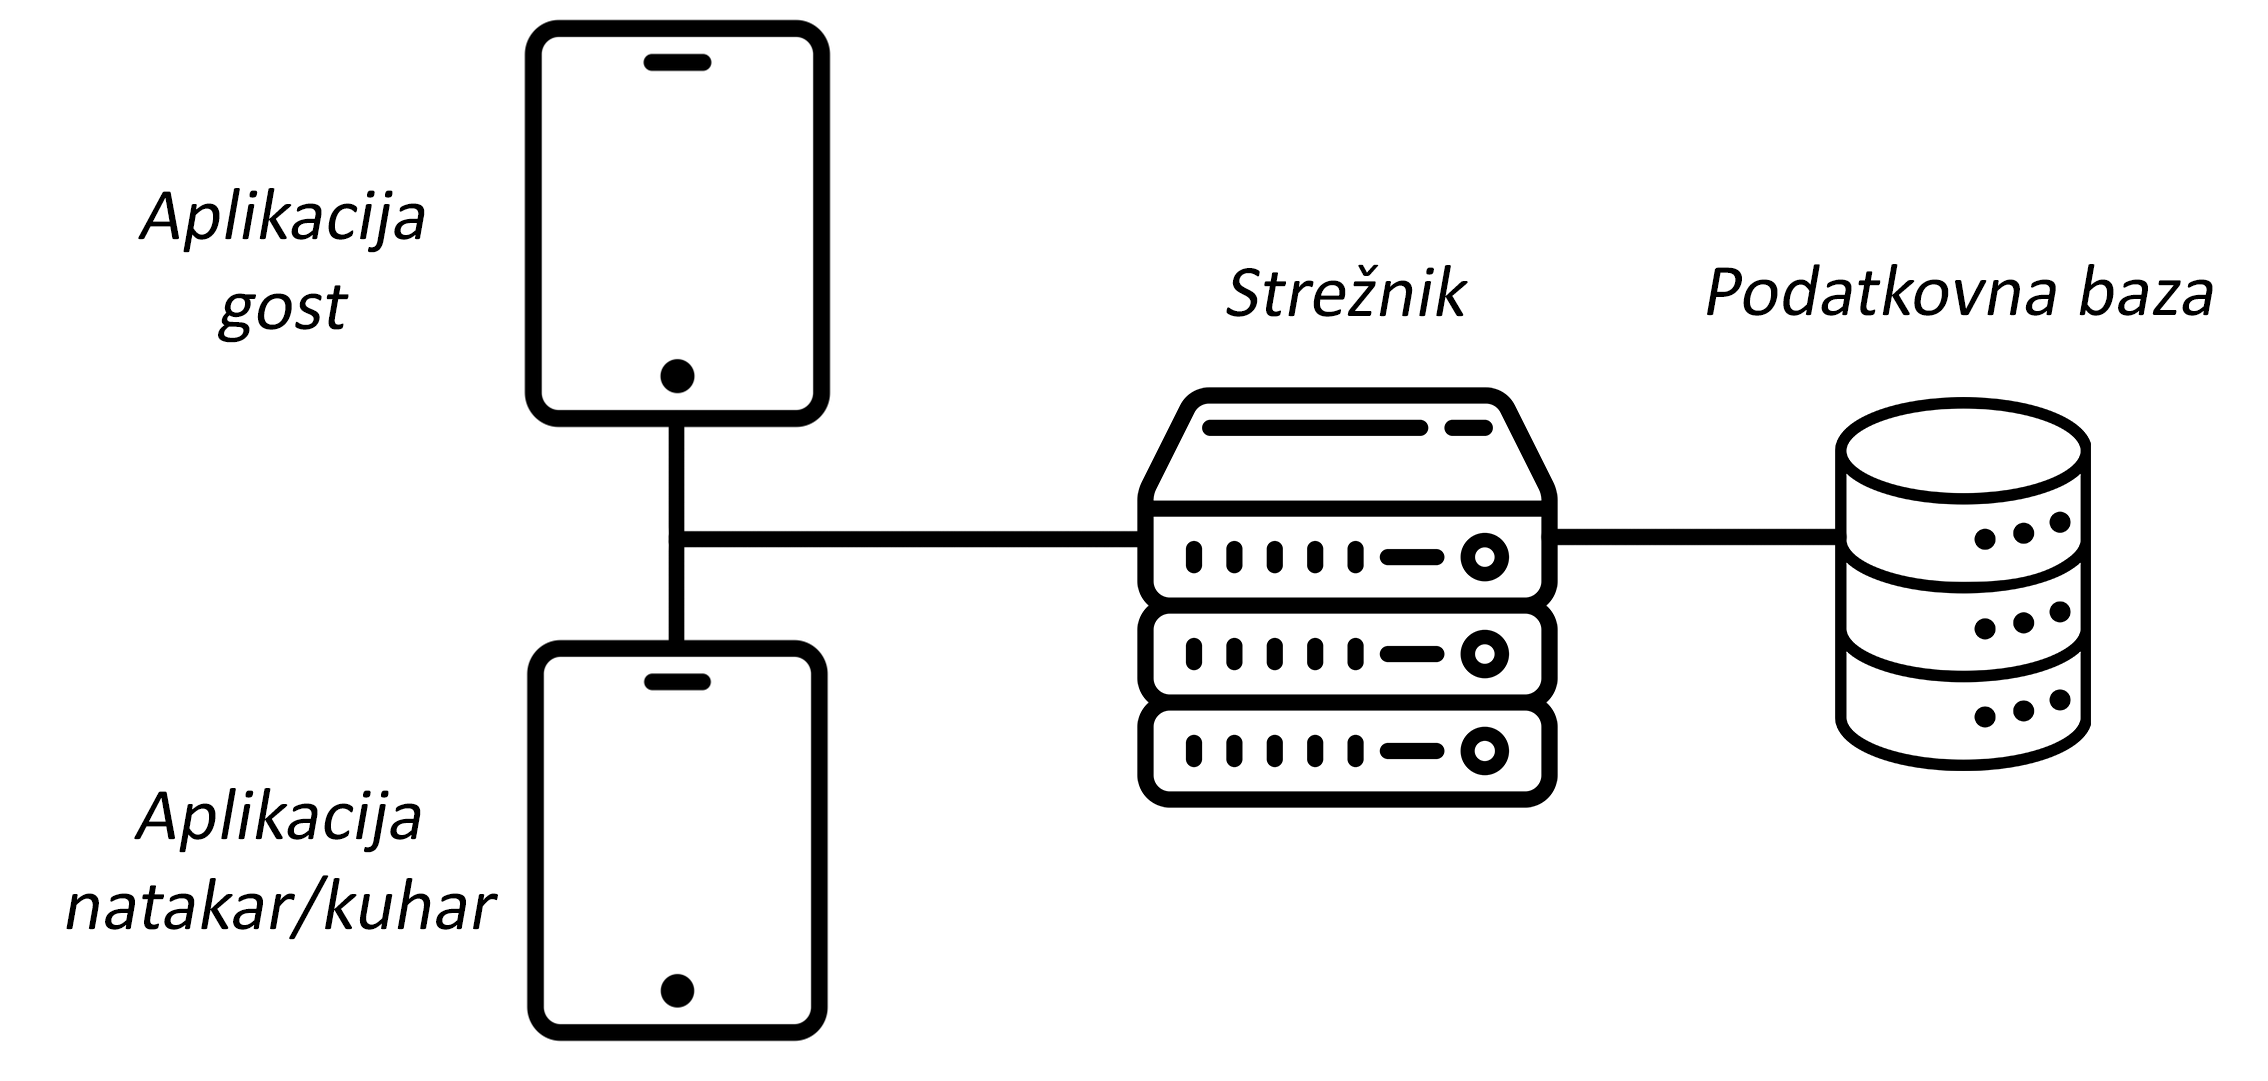
\includegraphics[width=10.8cm]{Skica1-new.png}
\caption{Visokonivojska arhitektura}
\label{StrukApk}
\end{figure}


\section{Podatkovna baza}
Na podlagi predvidenih zahtev oziroma funkcionalnosti, ki jih bo imela spletna aplikacija, smo najprej izdelali logičen podatkovni model (slika~\ref{Database_physical}). Podatkovna baza je sestavljena iz šestih tabel, ki so: \textit{ProductType, Product,  Order, ProductOrder, Table, User}. 

\begin{figure}[!htb]
\centering
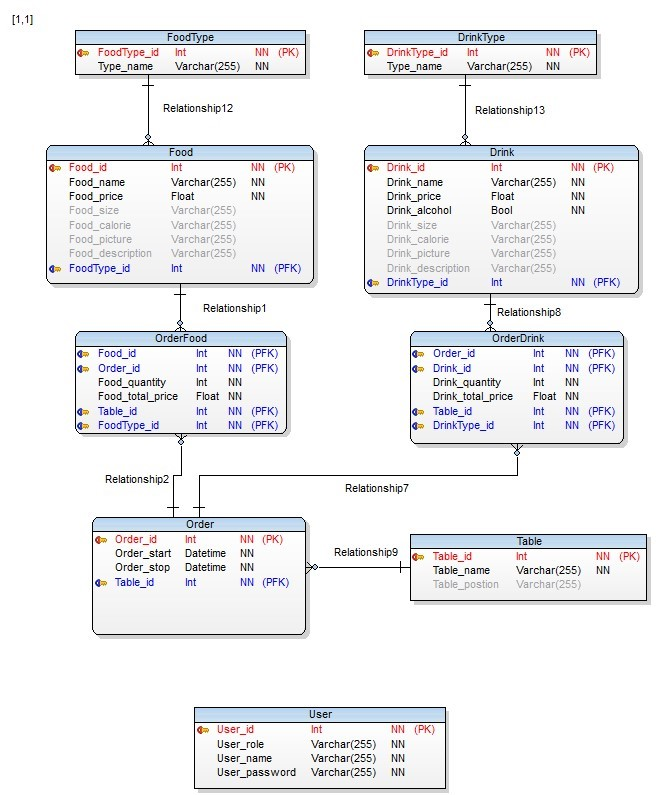
\includegraphics[width=12cm]{Database_physical}
\caption{Logični podatkovni model}
\label{Database_physical}
\end{figure}

Tabela \textit{ProductType} je namenjana zapisom za vrste jedi (predjed, glavna jed, sladica) in pijač (sokovi, piva, vina, itd.). Sestavljena je iz atributov: \textit{ID}, \textit{Name} in \textit{Type}. Atribut \textit{Type} je namenjen razlikovanju hrane in pijače v naročilu.

Tabela \textit{Product} je namenjena opisu hrane in pijače ter je sestavljena iz atributov: \textit{ID}, \textit{Name}, \textit{Price}, \textit{Size}, \textit{Calorie}, \textit{Picture} in \textit{Description}. V vrednost atributa \textit{Picture} se zapiše ime slike, ki se prikaže v aplikaciji.

Tabela \textit{Order} je namenjena zapisovanju naročil in njihovih podrobnosti. Sestavljena je iz atributov: \textit{ID}, \textit{Start}, \textit{End}, \textit{OrderStatus}, \textit{CookStatus} in \textit{Payment}. Vsebuje tudi tuji ključ od tabele \textit{Table}, ki določa, na katero mizo je vezano naročilo. Atributa \textit{OrderStatus} in \textit{CookStatus} sta definirana kot naštevalni podatkovni tip (angl. Enumerated Type, ENUM), ki sporočata status naročila med vlogami.

Tabela \textit{ProductOrder} je namenjena količini in končni ceni hrane in pijače v naročilu. Sestavljena je iz atributov: \textit{TotalPrice} in \textit{Quantity}. Zapis ne obstaja, če nima definiranega naročila. Tabela je nastala zaradi razmerja M : N, t. i. mnogo-proti-mnogo, med tabelo \textit{Product} in \textit{Order}.

Tabela \textit{Table} je namenjena označevanju miz v restavracijah. Sestavljajo jo atributi: \textit{ID}, \textit{Name} in \textit{Position}, v katerega se lahko podrobneje opiše lokacija mize.

Tabela \textit{User} je namenjena le natakarjem in kuharjem. Sestavljena je iz atributov: \textit{ID}, \textit{Role}, \textit{Name} in \textit{Password}. 

Strukturo podatkovne baze smo definirali s pomočjo programa Toad Data Modeler. To je orodje za izdelavo visokokakovostnih podatkovnih modelov \cite{Toad_Data_Modeler}. Omogoča izdelavo logičnih in fizičnih podatkovnih modelov, kar pripomore k lažjemu razumevanju in razvijanju podatkovne baze. Njegova najboljša funkcionalnost je, da lahko generiramo SQL kodo v različne podatkovne sisteme, npr. MySQL, Ingres, Microsoft Azurem, Microsoft Access in Mircrosoft SQL Server.

Fizični podatkovni model smo implementirali v sistemu za upravljanje podatkovne baze (angl. Database Management System, DBMS) MySQL. To je eden od odprtokodnih sistemov za upravljanje podatkovnih baz, ki za delo s podatki uporablja jezik SQL (angl. Structured Query Language) \cite{MySQL}. Napisan je v programskem jeziku C in C++ in deluje v vseh modernih operacijskih sistemih (Windows, Linux, IOS in drugih).


\section{Strežnik}
Strežnik predstavlja vmesnik med podatkovno bazo in odjemalcem. Najpomembneje je, da je sistem zanesljiv, saj odjemalec brez strežnika ne more delovati. Izbrali smo arhitekturo REST (angl. Representational State Transfer) zaradi načel, ki so opisana spodaj \cite{RESTAPI}. Sama arhitektura omogoča, da odjemalec z zahtevami pridobiva podatke od strežnika, ki jih s pomočjo povezav URI (angl. Uniform Resource Identifier) oglašuje na relativnih povezavah. Strežnik smo napisali v programskem jeziku Python z vključitvijo knjižnic Flask, MySQL, SocketIO in CORS. Načela arhitekture REST so sledeča:

1.) Odjemalec-strežnik (angl. Client-server) zahteva ločitev odjemalca od strežnika, kar odjemalcu onemogoča neposredno povezljivost s podatkovno bazo in s tem poenostavi razširljivost uporabniškega dela. Strežnika ne zanima uporabniški vmesnik ali podatki, tako da je enostavnejši in bolj prilagodljiv za uporabo. Tako se lahko uporabniški in strežniški del razvijata ali zamenjujeta neodvisno. V aplikaciji imamo dva različna odjemalca (gost in natakar/kuhar), kar za strežnik ne predstavlja nobenih omejitev, razen pri podatkovni bazi, ki omejuje število hkratnih poizvedb. V naši aplikaciji te omejitve nismo presegli.

2.) Brez stanja (angl. Stateless) morajo biti vse interakcije med strežnikom in odjemalcem. Strežnik ne sme shranjevati nobenih stanj oziroma mora vsako zahtevo odjemalca obravnavati kot popolnoma novo. V programski kodi strežnika je dobro razvidno, da ne uporabljamo nobenih globalnih spremenljivk. Vsi podatki, ki so potrebni, da strežnik odgovori na zahtevo HTTP (angl. Hypertext Transfer Protocol), se nahajajo bodisi v podatkovni bazi bodisi jih odjemalec na strežnik posreduje z zahtevkom.

3.) Predpomnjenje (angl. Cachable) prinaša izboljšanje zmogljivosti za odjemalca in omogoča razširljivost strežnika, ker se obremenitev zmanjša. V aplikacijah REST se predpomnjenje uporabi za vire, ki to potrebujejo. V naši aplikaciji tega nismo uporabili, saj nimamo tako zahtevnih virov.

4.) Večslojni sistem (angl. Layered system) je sestavljen iz hierarhičnih slojev, kjer npr. za vmesnik API (angl. Application Programming Interface) uporabimo strežnik A, za shranjevanje podatkov strežnik B ter strežnik C za avtenticiranje zahtev. S tem odjemalec ne more ugotoviti, ali komunicira s končnim strežnikom ali posrednikom.

5.) Izvajanje programske kode na zahtevo (angl. Code on demand) je opcijsko načelo. Strežnik na zahtevo odjemalca pošlje oziroma izvede programsko kodo za odjemalca. To smo vpeljali s pomočjo spletnih vtičnikov (angl. Websocket), ki so podrobneje opisani spodaj.

6.) Enotni vmesnik (angl. Uniform interface) med strežnikom in odjemalcem. Vsak vir mora vsebovati povezavo, ki kaže na svoj relativni URI. Odjemalec te vire pridobi od strežnika v obliki zahtev, ki so lahko GET, POST, PUT ali DELETE. Za predstavitev virov se lahko uporabi poljuben format, vendar sta najpogostejša XML (angl. Extensible Markup Language) in JSON (angl. JavaScript Object Notation).

Knjižnica Flask nam je poenostavila izdelavo strežnika, saj gre ze eno izmed najpriljubljenejših spletno aplikacijskih vmesnikov (angl. Framework) \cite{Flask}. Zasnovan je tako, da omogoča hiter in enostaven začetek z možnostjo razširitve na zapletene aplikacije. Flask je prvotno zasnoval in razvil Armin Ronacher kot prvoaprilsko šalo leta 2010. Kljub taki predstavitvi je Flask postal izjemno priljubljen kot alternativa projektom, narejenim v spletnem ogrodju Django.

Vsaka relativna povezava URI na strežniku predstavlja svoj vir podatkov iz podatkovne baze. Podatki so odjemalcu na voljo v podatkovnem formatu JSON. Strežnik s pomočjo knjižnice MySQL najprej prebere podatke iz podatkovne baze in jih predstavi na določeni relativni povezavi URI, ki jo določimo mi. Na sliki~\ref{Drinks_DB_function} je prikazana funkcija za branje podatkov iz podatkovne baze, kjer spemenljivka \textit{query} predstavlja poizvedbeni stavek. Slika~\ref{Drinks_URI} prikazuje uporabo te funkcije in relativne poti \textit{drinks}. Strežnik vsebuje 34 relativnih povezav URI in 600 vrstic programske kode.


\begin{figure}[!htb]
\begin{center}
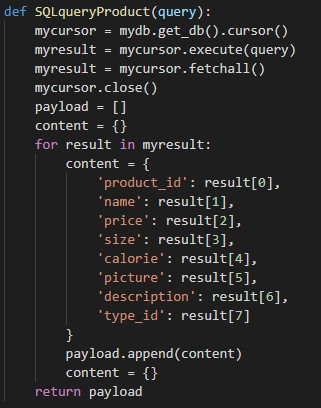
\includegraphics[width=0.5\textwidth]{drinks_1.jpg}
\caption{Funkcija, ki prebere podatke iz podatkovne baze}
\label{Drinks_DB_function}
\end{center}
\end{figure}

\begin{figure}[!htb]
\begin{center}
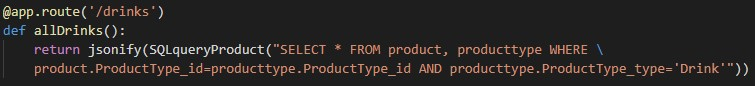
\includegraphics[width=14cm]{drinks_2.jpg}
\caption{Funkcija, ki na relativno stran \textit{drinks} servira podatke}
\label{Drinks_URI}
\end{center}
\end{figure}

Tako smo dobili vmesnik, ki na zahtevo odjemalca odgovori s podatki v formatu JSON. Na sliki~\ref{ServerEX} je primer zahtevka v programu Postman, ko odjemalec zahteva podatke vseh pijač iz podatkovne baze (metoda GET protokola HTTP). Strežnik omogoča tudi sprejemanje podatkov z metodami PUT in POST. Mi smo uporabili metodo POST za posredovanje podatkov, ki so potrebni za zapis v podatkovno bazo, na strežnik. Spremljanje zahtevkov na strežniku je mogoče v konzolnem vmesniku (angl. Command-Line Interface, CLI), ki se uporablja pri zagonu strežnika (slika~\ref{ServerEX2}).

\begin{figure}[!htb]   
\begin{center}
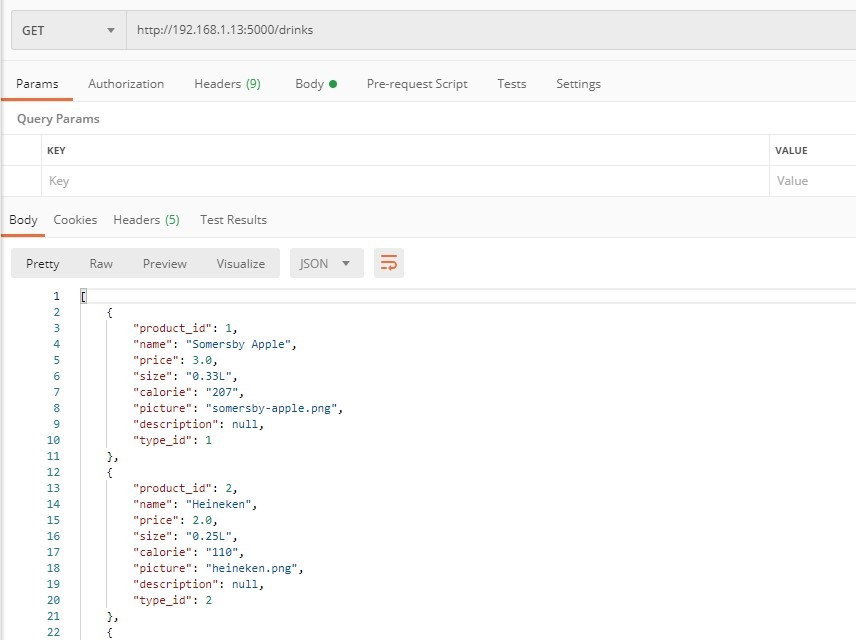
\includegraphics[width=10cm]{Server_example.jpg}
\caption{Primer serviranja podatkov na strežniku s programom Postman}
\label{ServerEX}
\end{center}
\end{figure}

\begin{figure}[!htb]
\centering
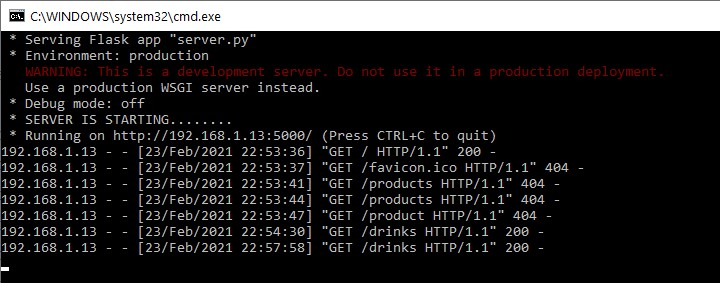
\includegraphics[width=13cm]{Server_example_2.jpg}
\caption{Primer spremljanja zahtevkov, ki prihajajo na strežnik}
\label{ServerEX2}
\end{figure}

Za potrebe pridobivanja podatkov v realnem času za odjemalca, smo uporabili spletni vtičnik SocketIO. Implementirali smo ga na strežniku in odjemalcu. Zagotavlja dvosmerno komunikacijo oziroma komunikacijo na podlagi dogodkov. Deluje na vseh platformah, brskalnikih ali napravah. Uporabili smo ga zaradi medsebojnega obveščanja odjemalcev o spremembah v podatkovni bazi. Uporabili smo funkcijo \textit{emit}, ki omogoča dodajanje podatkov in izbiranje načina razpršenega oddajanja (angl. Broadcast). To pomeni, da ob oddajanju strežnika vsi prejemajo te informacije. Gre predvsem za splošne podatke, tako da ne more priti do zlorabe. Na primer: ob gostovi spremembi naročila se te razlike preverijo na strežniku in vpišejo v podatkovno bazo, natakarja pa se o tem obvesti s funkcijo \textit{emit}, ki vsebuje številko naročila, v katerem je prišlo do sprememb. 
	

Aplikacija omogoča urejanje določenih podatkov, zato smo morali zagotoviti ustrezno varnost za njihovo urejanje. Prva raven varnosti je avtorizacija odjemalca. Zahtevki, ki se pošiljajo na strežnik, morajo biti omogočeni samo avtoriziranim odjemalcem. Zato smo uporabili piškotke HTTP (angl. Cookies), ki so izdelani za spletne brskalnike in so namenjeni za sledenje, prilagajanje in shranjevanje informacij o posamezni seji uporabnika. Vsi piškotki so shranjeni pri odjemalcu in so kriptografsko zaščiteni pred morebitnimi nepooblaščenimi dostopi. S tem odjemalcu preprečujemo spreminjanje podatkov v piškotkih oz. lahko nedovoljene spremembe podatkov na strežniku zaznamo. Uporabili smo Flask-Login, ki omogoča vse funkcionalnosti za upravljanje uporabniških sej. 
Na sliki~\ref{Cookies} je prikazano delovanje piškotkov HTTP. Strežnik ob prvem zahtevku, torej ob uspešni prijavi, odjemalcu vrne piškotek. Odjemalec ob vsakem nadaljnjem zahtevku doda piškotek, s katerim strežnik overi zahtevo odjemalca.

\begin{figure}[!htb]
\begin{center}
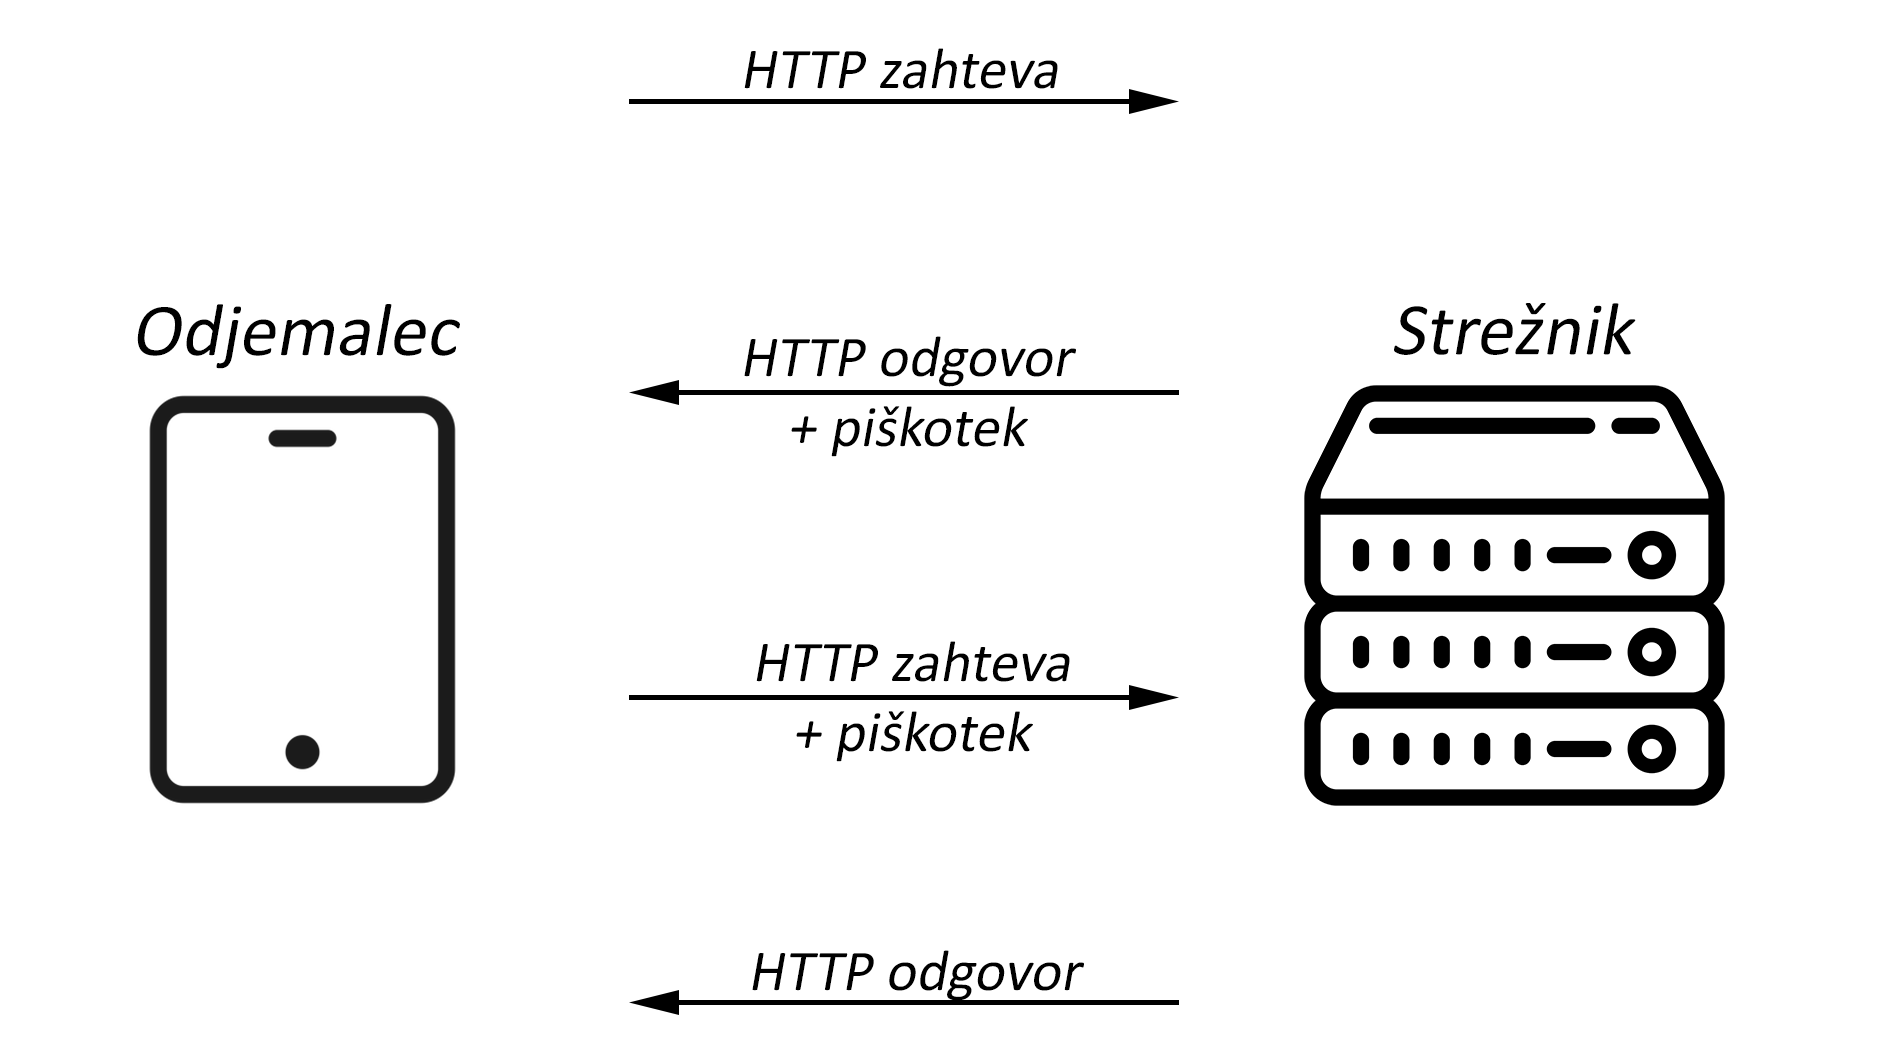
\includegraphics[width=13.5cm]{cookie-how1.png}
\caption{Delovanje piškotkov HTTP med odjemalcem in strežnikom}
\label{Cookies}
\end{center}
\end{figure}

\section{Odjemalec}

Odjemalca bi lahko implementirali v spletnih tehnologijah (HTML, CSS in JavaScript) ali pa v namenski mobilni aplikaciji. Odločili smo se za spletne tehnologije, kjer je glavnina odjemalca implementrana v programskem jeziku JavaScript s pomočjo ogrodja Vue.  Naredili smo odziven in reaktiven vmesnik, ki deluje v stvarnem času. Vue je eden izmed mnogih, kot npr. Angular, Ember, React, poznan pa je predvsem zaradi enostavnosti upravljanja in izvajanja testov. Vsem je skupna reaktivnost, vendar v drugačnem pomenu besede. Reaktivnost \cite{reaktivnost} je programska paradigma, ki nam omogoča, da se na deklarativni način prilagodimo spremembam. Tako deluje tudi reaktivnost v aplikacijah, kjer je podatek lahko vezan na več funkcij oziroma delov programske kode, ki se ob spremembi vrednosti posodobijo. Vue je namenjen izdelavi enostranskih aplikacij (angl. Single-Page Application, SPA), saj vsebuje samo eno datoteko HTML. To prednost smo izkoristili s pomočjo ostalih knjižnic, ki so nam omogočale enostavnejšo izdelavo aplikacije. Uporabili smo naslednje:
\begin{description}
\item[Vue CLI] velja kot standardno orodje za ekosistem Vue \cite{VueCLI}. Zagotavlja, da že pri gradnji novega projekta poveže različne dodatke med seboj. To razvijalcu omogoča, da se bolj osredotoči na programiranje in ne na njihovo povezovanje v projekt. Z uporabo vmesnika CLI se lahko izbere projekt, kjer so na voljo že privzete nastavitve, lahko pa se jih tudi nastavi po meri. Mi smo uporabili Vuex, Vue-Router, ESLint in Vuetify.
\item[Vuex] je knjižnica za shranjevanje vrednosti v aplikacijah Vue.js \cite{Vuex}. Služi kot centralizirana baza podatkov za vse komponente v aplikaciji. 
\item[Vue-Router] je uradni usmerjevalnik za Vue.js \cite{VueRouter}. Integrira se globoko z jedrom Vue.js, tako da poenostavi izdelavo aplikacij SPA. Usmerjevalnik je mišljen v smislu usmerjanja na druge komponente (angl. Component), ki v Vue.js predstavljajo druge poglede oziroma podstrani.
\item[ESLint] je orodje za prepoznavanje in poročanje o popravkih v programski kodi \cite{ESLint}. Cilj je narediti kodo preglednejšo in bolj urejeno, kar pripomore k izogibanju napakam.
\item[Vuetify] je eden izmed mnogih uporabniških vmesnikov, ki je zgrajen na vrhu Vue.js \cite{Vuetify}. V nasprotju z drugimi vmesniki je Vuetify enostaven za učenje z več stotimi komponentami, izdelanimi po specifikacijah Material Design.
\item[Vue-devtools] je zgolj dodatek v brskalniku, ki omogoča lažje sledenje delovanju aplikacije in detektiranju napak. 
\end{description}

Programsko izvedbo za odjemalca smo razdelili v tri vloge oziroma dve aplikaciji. Ena aplikacija je namenjena natakarjem in kuharjem, ločuje se s prijavnim oknom in videzom vmesnika. Druga aplikacija je namenjena samo gostom in je sestavljena iz več pogledov. Ločili smo jih zaradi varnosti, lažjega razvijanja in preglednosti, saj gre za dve popolnoma različni aplikaciji. Vse funkcionalnosti in delovanje ene in druge aplikacije so opisani v naslednjem poglavju.

Ena izmed pomembnih stvari pri obratovanju restavracije je čim hitrejša postrežba, ki jo je mogoče izboljšati s čim hitrejšo komunikacijo. Zato smo, enako kot za strežnik, uporabili spletni vtičnik SocketIO. Vključili smo ga v obeh aplikacijah, in sicer za oddajanje naročil, posodabljanje naročil, obveščanje gosta o stanju naročila itd. Najprej smo hoteli uporabiti samodejno osveževanje na določen časovni interval, vendar je uporaba spletnih vtičnikov hitrejša in učinkovitejša. Slika~\ref{socketioo1} prikazuje primer vtičnikov, ki so uporabljen za gosta.

\begin{figure}[!htb]
\begin{center}
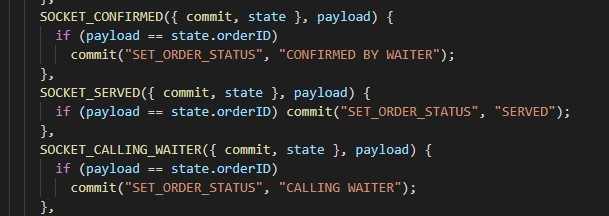
\includegraphics[width=11cm]{socketio_2.jpg}
\caption{Uporaba spletnih vtičnikov za gosta}
\label{socketioo1}
\end{center}
\end{figure}

Za potrebe pridobivanje podatkov za odjemalca smo uporabili Axios, ki je namenjen procesiranju zahtevkov  HTTP. To pomeni, da podatke, ki jih oglašuje strežnik, s pomočjo te knjižnice pridobimo za odjemalca (slika~\ref{axios_1}). 

\begin{figure}[!htb]
\begin{center}
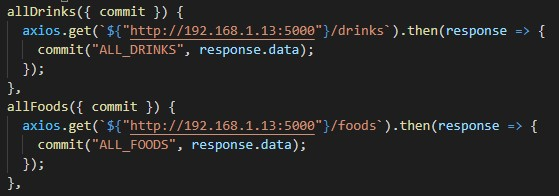
\includegraphics[width=11cm]{axios_1.jpg}
\caption{Način uporabe Axios v aplikaciji za gosta}
\label{axios_1}
\end{center}
\end{figure}


\chapter {Delovanje aplikacije}
Delovanje aplikacije smo testirali v testnem okolju. Uporabili smo osebni računalnik, na katerem smo postavili podatkovno bazo MySQL, strežnik in aplikaciji za gosta in natakarja/kuharja. Slika~\ref{Program1} prikazuje testno okolje.

\begin{figure}[!htb]
\begin{center}
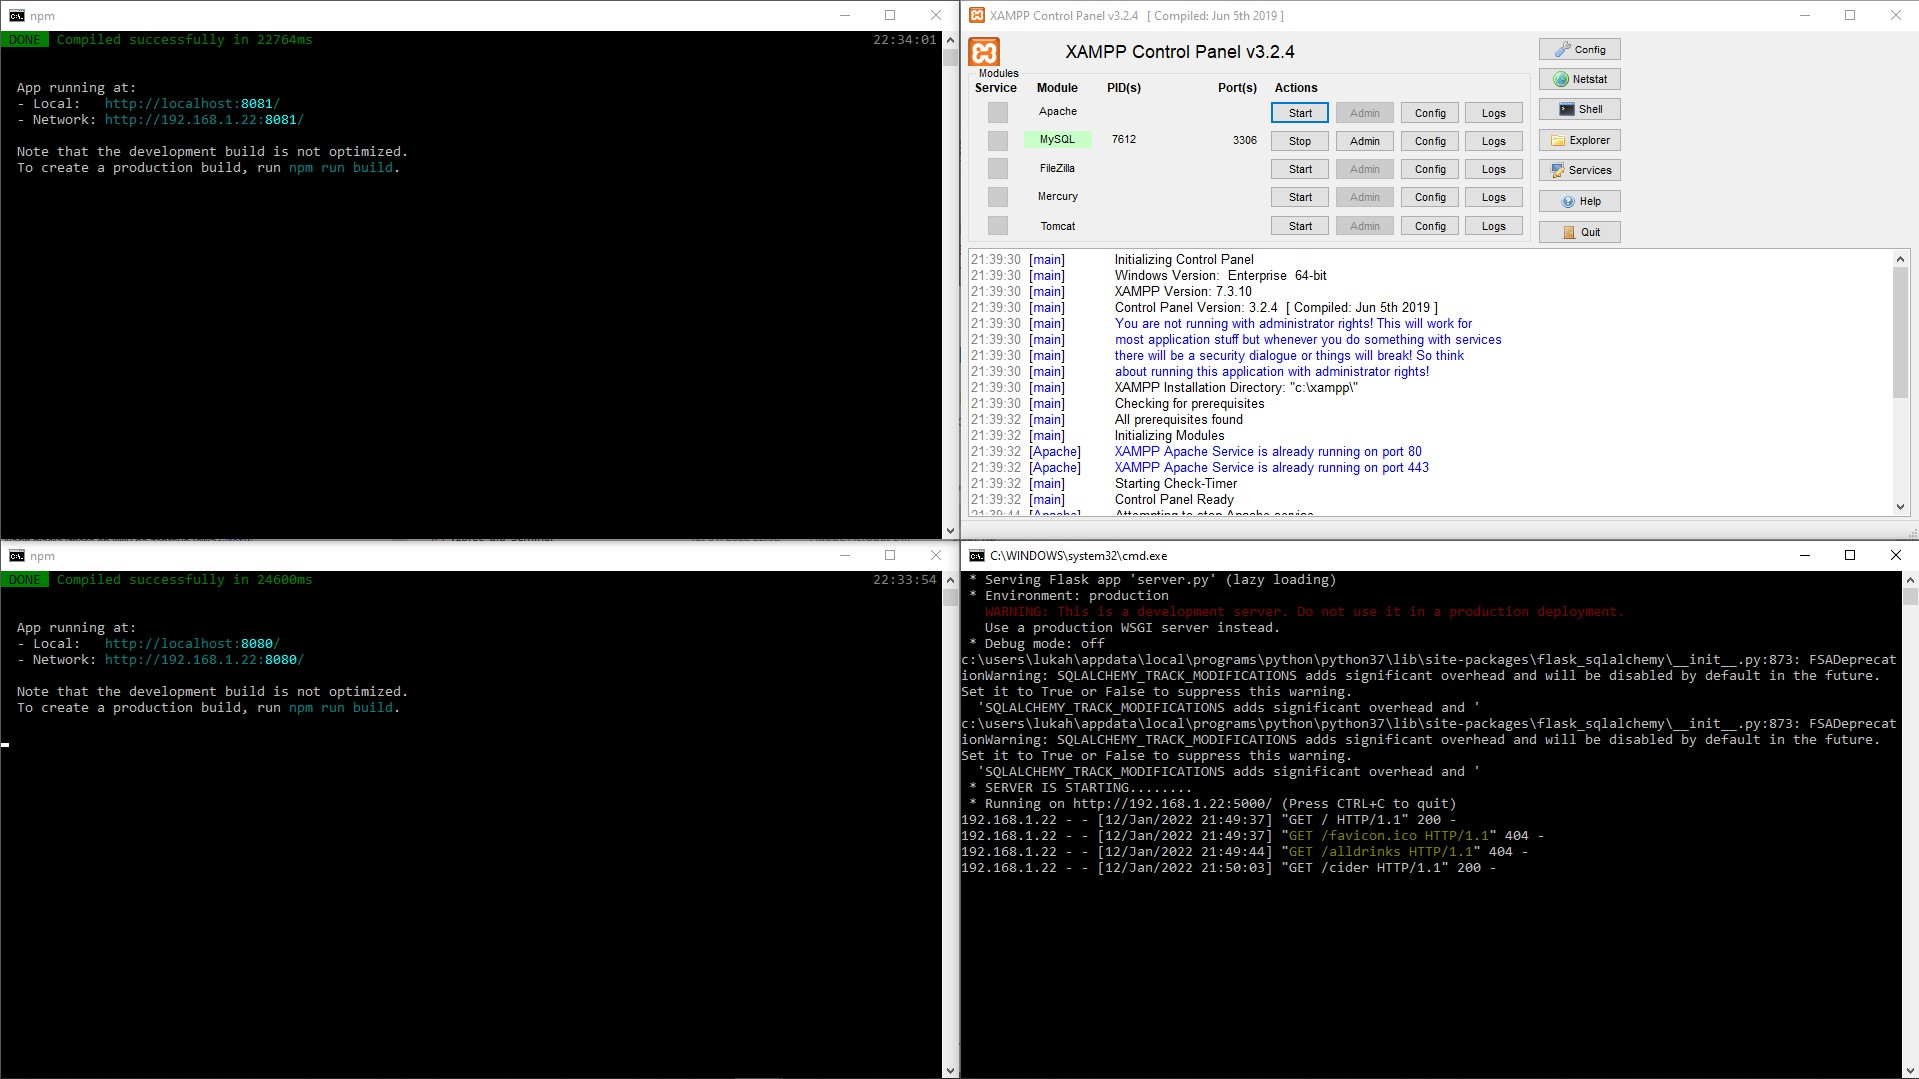
\includegraphics[width=14cm]{Programi.jpg}
\caption{Testno okolje na osebnem računalniku}
\label{Program1}
\end{center}
\end{figure}


\section{Vmesnik za gosta}
Začetni pogled vmesnika za gosta vsebuje napis za dobrodošlico (slika~\ref{Gost_zac}), ki bi ga lahko zamenjali oglaševanje, predstavitev restavracije ali karkoli bi si potencialni kupec zaželel imeti. V zgornjem desnem kotu se nahajta gumb \textit{call waiter} za priklic natakarja in števec skupne cene artiklov v nakupovalni košarici. Gumb \textit{call waiter} je namenjen gostom, ki aplikacije ne želijo uporabljati, ali v primeru pomoči, če ima gost kakšna vprašanja ali pride do kakršnihkoli težav. V spodnjem levem kotu se nahajata status in identifikacijska številka naročila. 
Zavihki na levi strani predstavljajo seznam vseh vrst hrane in pijače, ki kažejo na podstrani ponudbe restavracije (slika~\ref{Gost_3}). Gostu to predstavlja ponudbo, med katero izbira pri dodajanju hrane in pijače v nakupovalno košarico.

\begin{figure}[!htb]
\centering
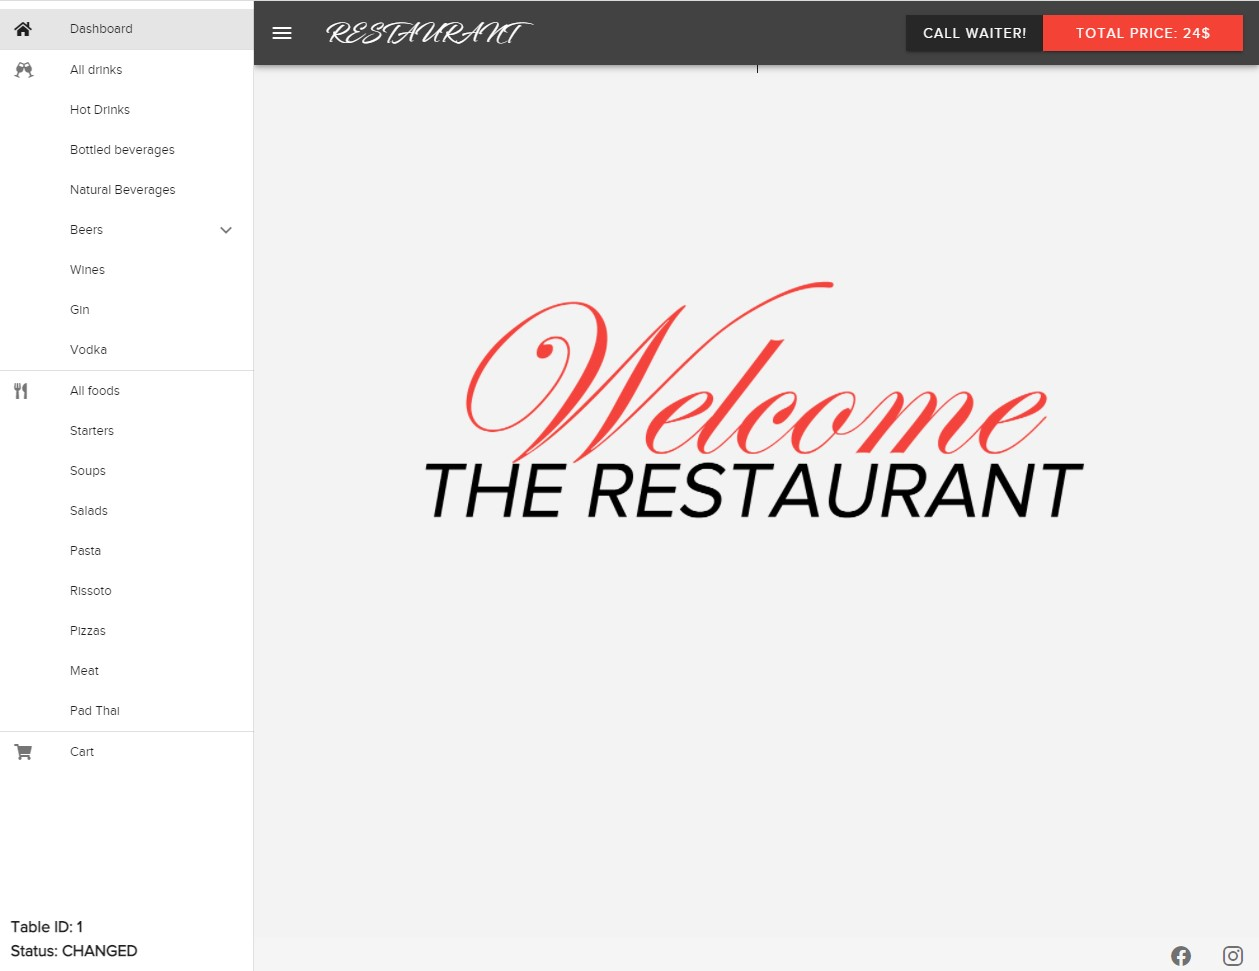
\includegraphics[width=13.7cm]{gost_zacetek.jpg}
\caption{Začetni pogled vmesnika za gosta}
\label{Gost_zac}
\end{figure}

\begin{figure}[!htb]
\centering
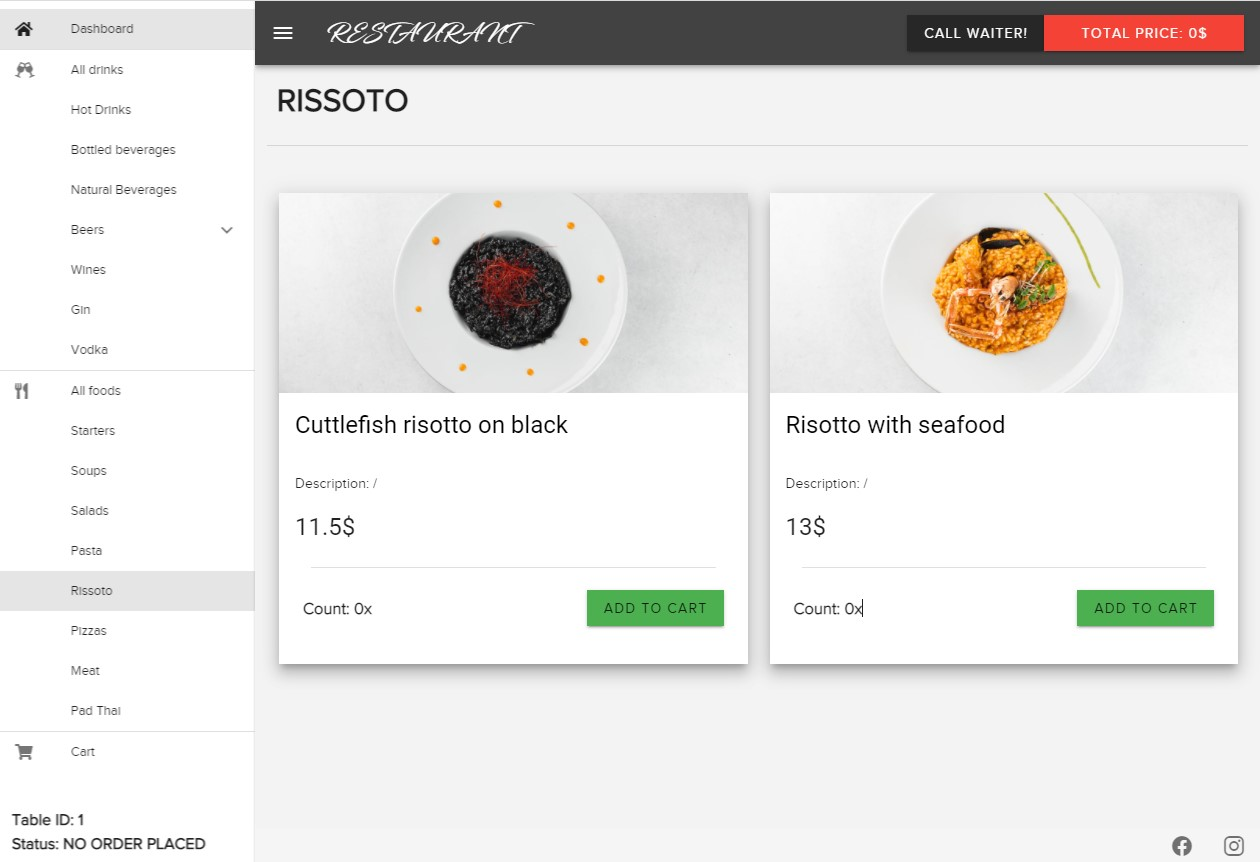
\includegraphics[width=13.7cm]{customer_1.jpg}
\caption{Seznam artiklov znotraj vrste rižot}
\label{Gost_3}
\end{figure}
Vsaka hrana ali pijača vsebuje sliko, ime, opis in ceno. Poleg tega vsebuje še gumb \textit{add to cart} (dodaj v košarico), ki ob kliku izgine in prikaže tri nove gumbe \textit{+} (povečaj količino), \textit{–} (zmanjšaj količino) in \textit{remove} (odstrani). Nakupovalna košarica oziroma \textit{cart} je skupno mesto vse hrane in pijače v seznamu za naročilo (slika~\ref{Gost_4}). Vse slike hrane in pijače so shranjene v datotečnemu sistemu spletnega strežnika. Naročilo se odda s klikom na gumb \textit{place order}, ki gosta preusmeri na prvo stran in obvesti s pojavnim sporočilom, prikazanim na sliki~\ref{Gost_5}. Ko je naročilo oddano, lahko gost ponovno dodaja hrano in pijačo v košarico, vendar je že oddani hrani in pijači onemogočeno zmanjšanje količine ali brisanje. Naročilo je sprejeto, ko ga natakar potrdi, kar spremeni status naročila in prikaže pojavno sporočilo, predstavljeno na sliki~\ref{Gost_6}. Če natakar uredi naročilo, ga mora gost pregledati in ponovno oddati. Tudi v tem primeru je gost obveščen s statusom in pojavnim sporočilom, vidnim na sliki~\ref{Gost_8}. Naročilo se zaključi s klikom na gumb \textit{request receipt}, ki odpre pojavno okno (slika~\ref{Gost_7}) za izbiro načina plačila.

\begin{figure}[!htb]
\centering
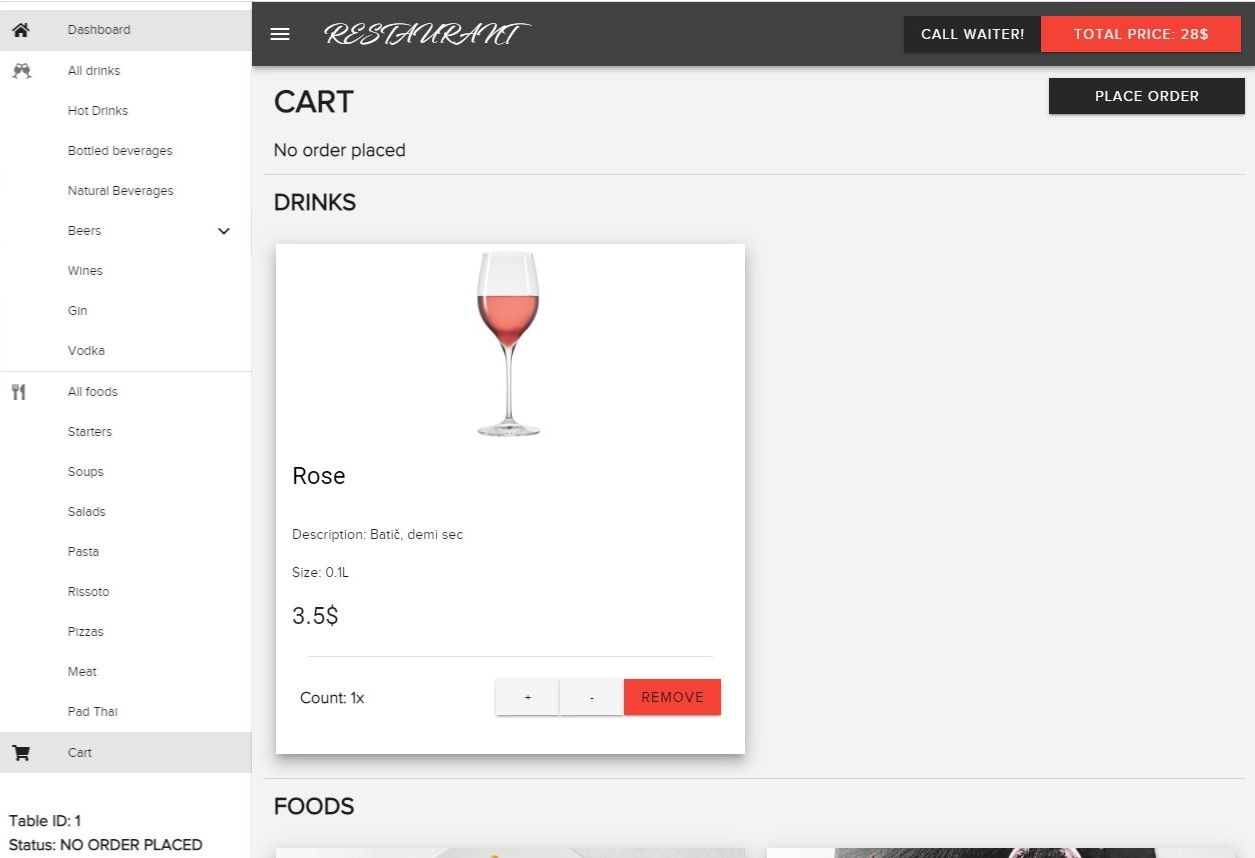
\includegraphics[width=13.7cm]{customer_2.jpg}
\caption{Primer naročila}
\label{Gost_4}
\end{figure}
\begin{figure}[!htb]
\centering

\includegraphics[width=11cm]{gost_5.jpg}
\caption{Pojavno sporočilo ob uspešni oddaji naročila}
\label{Gost_5}
\end{figure}
\begin{figure}[!htb]
\centering

\includegraphics[width=11cm]{gost_6.jpg}
\caption{Pojavno sporočilo ob natakarjevi potrditvi naročila}
\label{Gost_6}
\end{figure}
\begin{figure}[!htb]
\centering
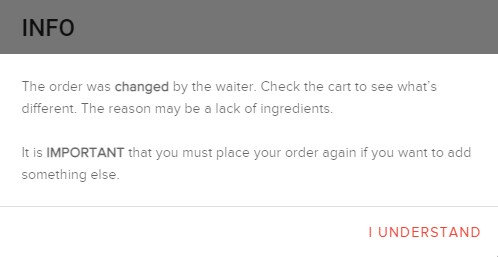
\includegraphics[width=11cm]{gost_8.jpg}
\caption{Pojavno sporočilo ob natakarjevi ureditvi naročila}
\label{Gost_8}
\end{figure}
\begin{figure}[!htb]
\centering

\includegraphics[width=11cm]{gost_7.jpg}
\caption{Pojavno okno z možnostjo izbire načina plačila}
\label{Gost_7}
\end{figure}

\clearpage
\section{Vmesnik za natakarja in kuharja}
Začetni pogled vmesnika je enak za natakarja in kuharja, saj gre za skupno aplikacijo, kjer se pogledi razlikujejo glede na vlogo uporabnika, ki je določena v podatkovni bazi. Nismo naredili ločene aplikacije, saj ni bilo potrebe, funkcije za oba uporabnika so namreč zelo podobne. Slika~\ref{NatKuh_zac} prikazuje prijavno okno. Po prijavi natakarja ali kuharja se uporabniško ime izpiše v levem spodnjem kotu. Na zgornji levi strani se prikaže zavihek z dvema podstranema in odjavnim gumbom \textit{sign out}. Prva podstran, imenovana \textit{dashboard}, ali prva stran ob uspešni prijavi prikazuje napis za hitrejšo razlikovanje med vlogami. Natakar ima v desnem zgornjem kotu še števec čakajočih in zaključenih naročil.
\begin{figure}[!htb]
\centering
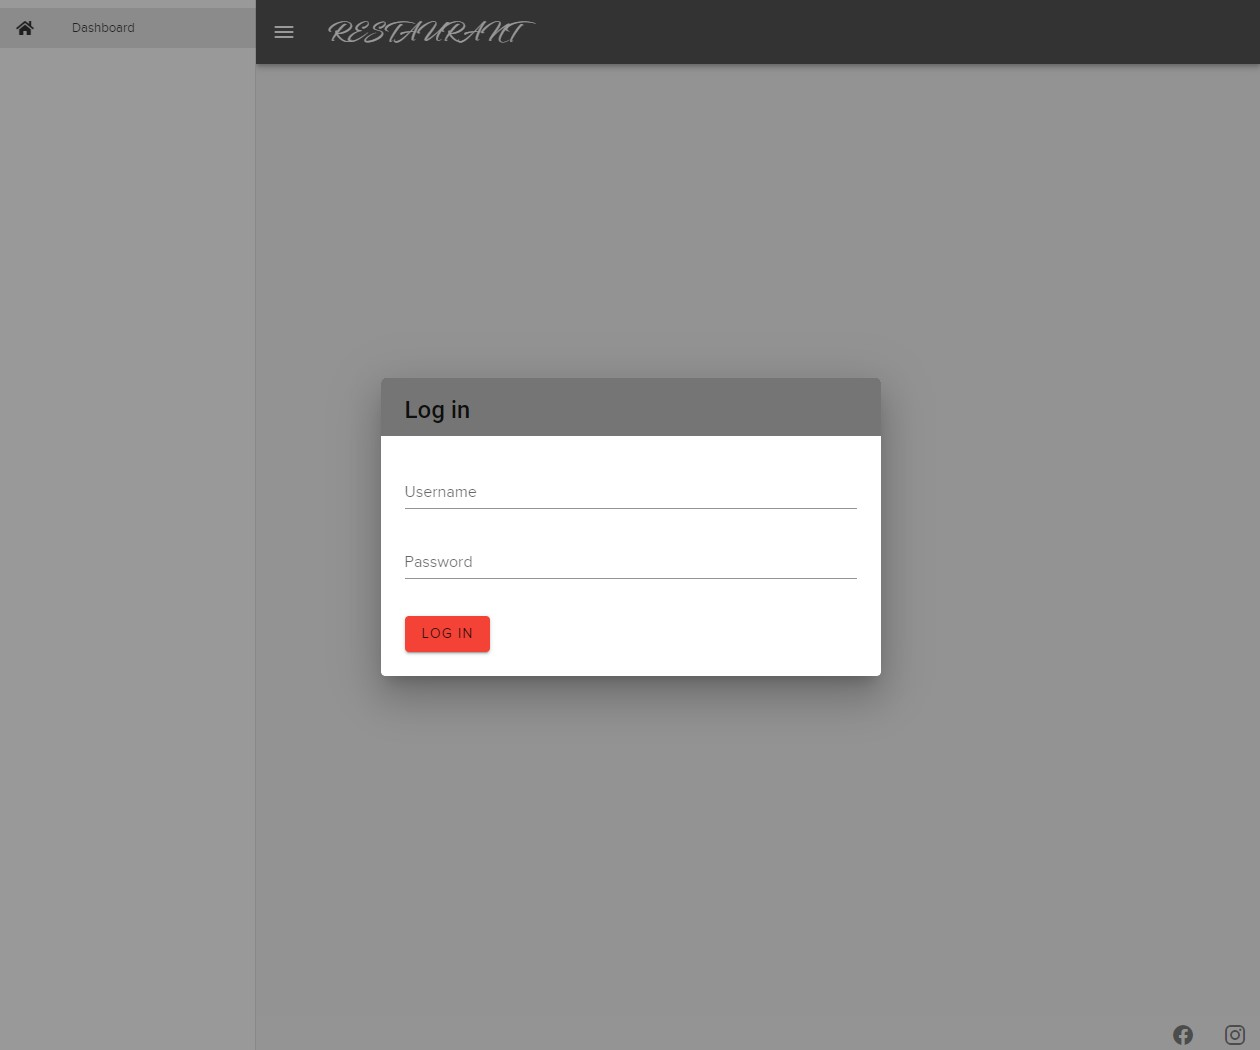
\includegraphics[width=13.7cm]{prijavno.jpg}
\caption{Prijavno okno za natakarja in kuharja}
\label{NatKuh_zac}
\end{figure}


Natakarju se v zavihku \textit{all orders} pojavijo vsa nezaključena naročila (slika ~\ref{Natakar_2}). Vsako naročilo vsebuje naslednje podatke: identifikacijska številka naročila, čas oddaje naročila, status naročila, status kuharja, način plačila in številka mize. Izvaja lahko popoln nadzor nad naročili, vendar ob vsaki izvedeni akciji obvesti gosta (slike pojavnih sporočil iz prejšnjega poglavja). Novo naročilo mora natakar najprej potrditi z gumbom \textit{confirm} ali urediti z gumbom \textit{check details} (slika~\ref{Natakar_3}). Natakar lahko ureja celotno naročilo, kar pomeni, da lahko spreminja količino hrane in pijače ali jo briše iz naročila. Ko zaključi urejanje, mora klikniti na gumb \textit{update order}. Celotno naročilo lahko potrdi šele, ko dobi kuharjevo potrditev o hrani. Ko je naročilo potrjeno, natakar čaka na kuharjevo potrditev o pripravi hrane, da jo lahko postreže. Natakar postreženo naročilo označi s klikom na gumb \textit{served}. Če gost zahteva račun, se natakarju izpiše način plačila v zadevi \textit{payment}. Naročilo se zaključi, ko natakar natisne račun s klikom na gumb \textit{invoice}.

\begin{figure}[!htb]
\centering
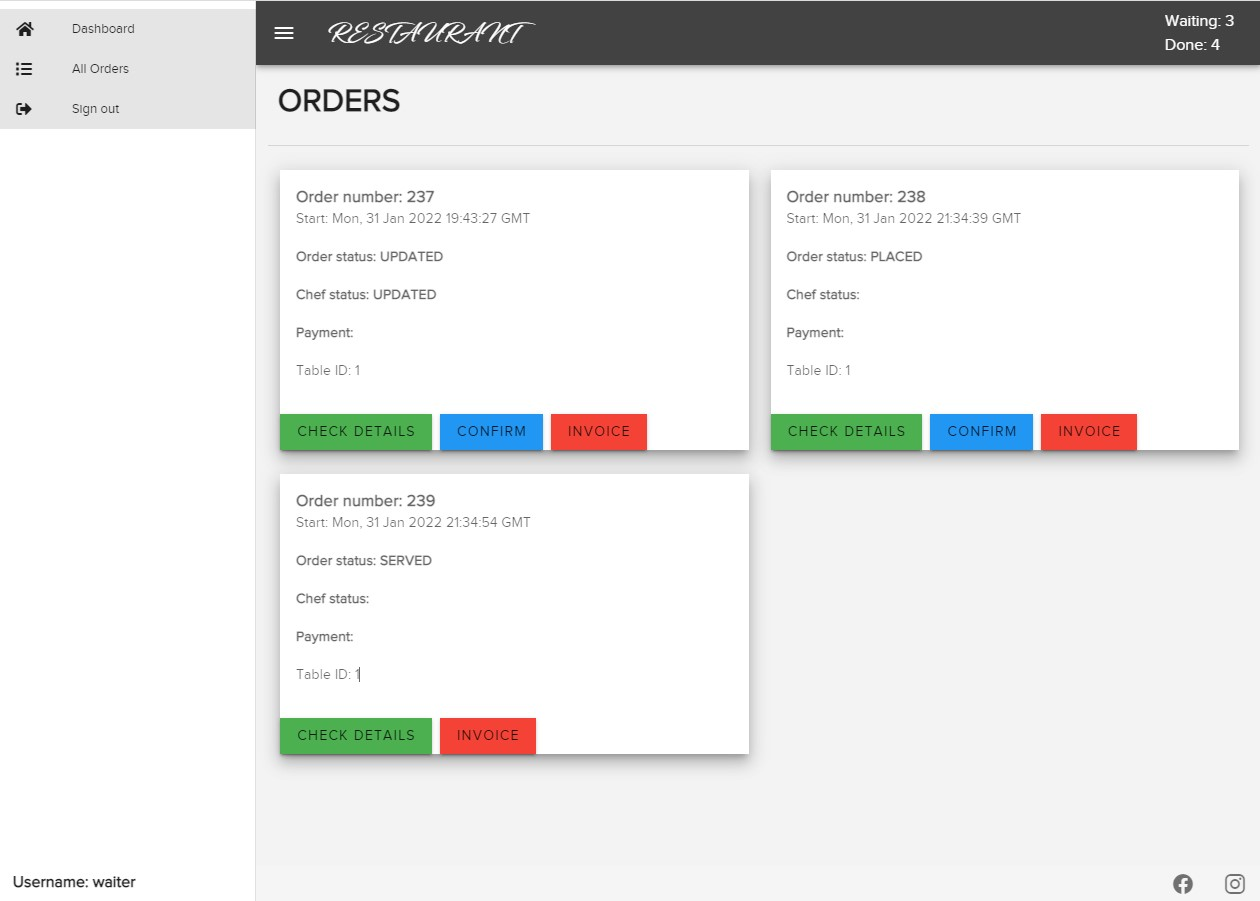
\includegraphics[width=13.3cm]{waiter_1.jpg}
\caption{Zavihek \textit{all orders}}
\label{Natakar_2}
\end{figure}

\begin{figure}[!htb]
\begin{center}
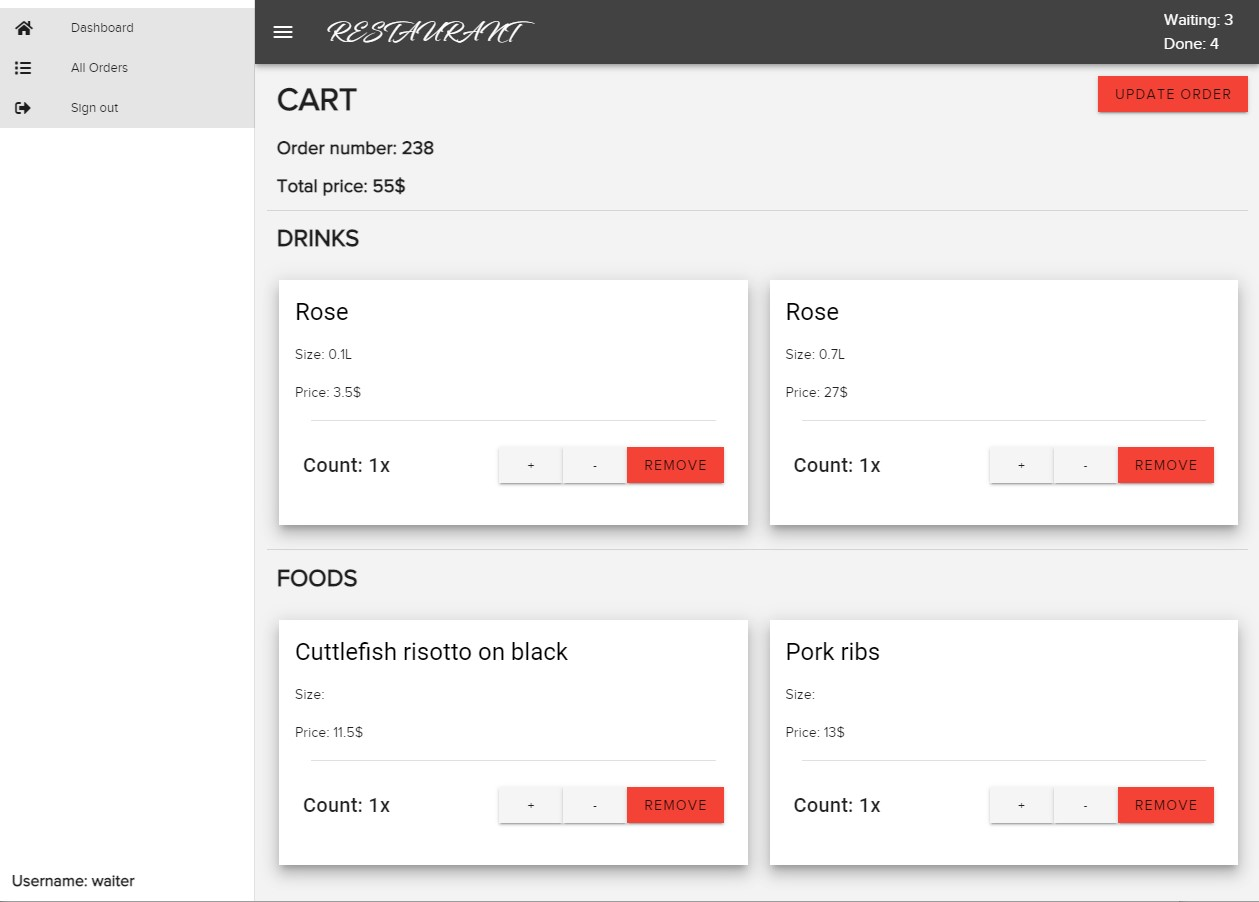
\includegraphics[width=13.7cm]{waiter_2.jpg}
\caption{Zavihek \textit{check details}}
\label{Natakar_3}
\end{center}
\end{figure}

Kuharju se v zavihku \textit{food orders} pojavijo vsa nezaključena naročila, ki vsebujejo hrano (slika ~\ref{Kuhar_4}). Vsako naročilo vsebuje naslednje podatke: identifikacijska številka naročila, čas oddaje naročila, status kuharja in številka mize. Kuhar mora naročilo najprej pregledati z gumbom \textit{check details} (slika  ~\ref{Kuhar_3}) ter ga sprejeti ali zavrniti z gumboma \textit{confirm} in \textit{decline}. Naročilo lahko kuhar zavrne, če mu zmanjka sestavin. Ko kuhar zaključi pripravo hrane, o tem obvesti natakarja s klikom na gumb \textit{done}, ki izbriše naročilo s seznama. Ob vsaki izvedeni akciji se pri vsakem naročilu spremeni status kuharja, ki je lahko: \textit{updated}, \textit{confirmed}, \textit{decline} in \textit{done}. Status \textit{updated} se uporabi, če gost k naročilu doda izdelke.

\begin{figure}[!htb]
\centering
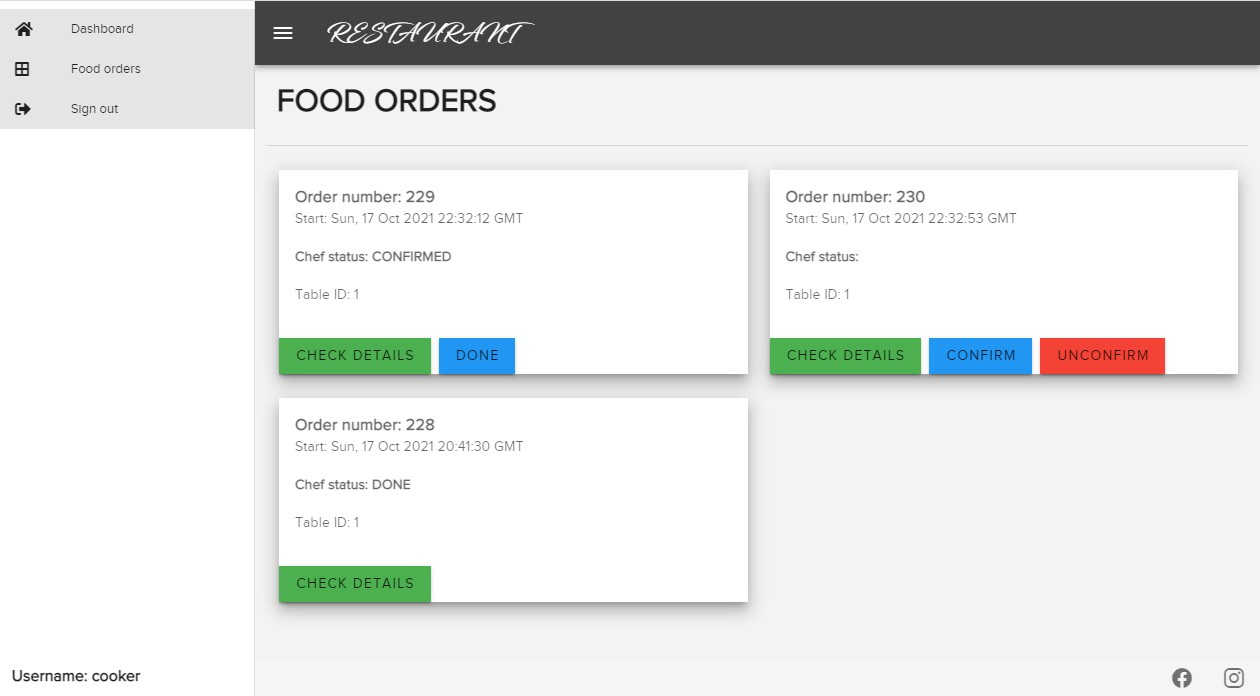
\includegraphics[width=13.7cm]{cooker_1.jpg}
\caption{Zavihek \textit{food orders}}
\label{Kuhar_4}
\end{figure}

\begin{figure}[!htb]
\centering
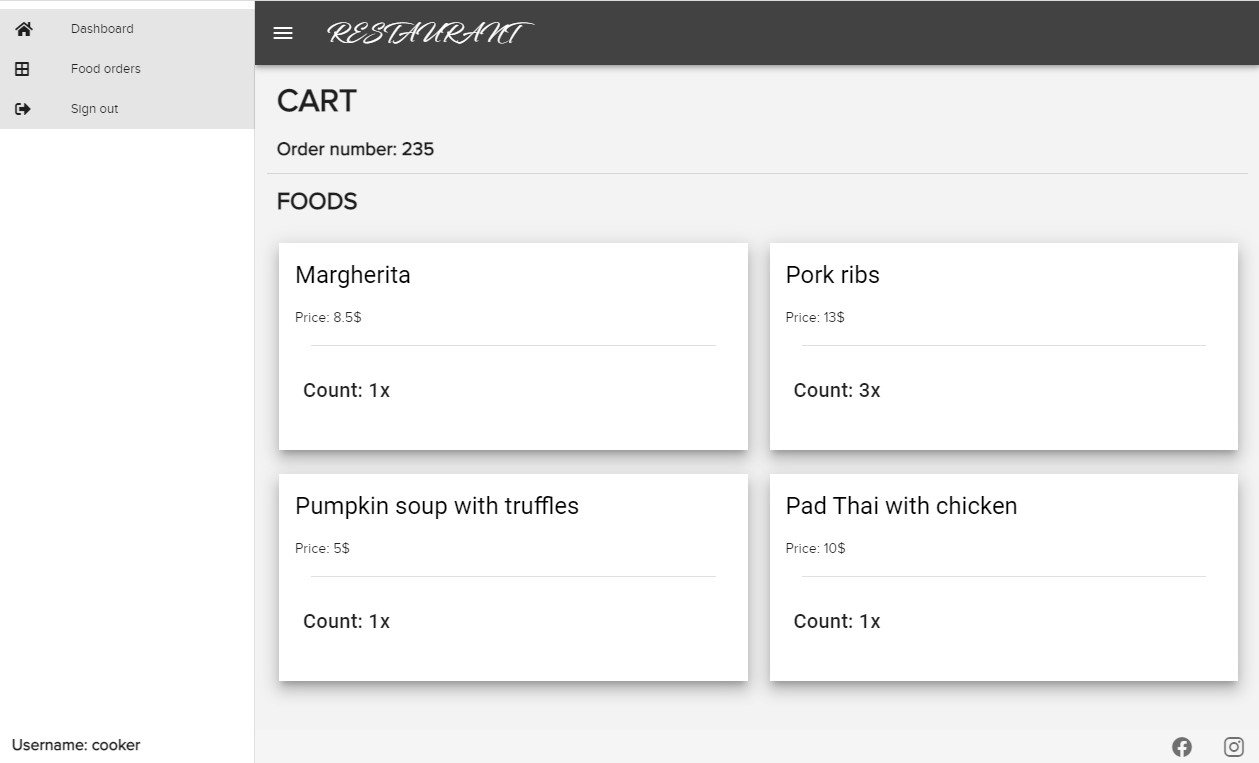
\includegraphics[width=13.7cm]{cooker_2.jpg}
\caption{Zavihek \textit{check details}}
\label{Kuhar_3}
\end{figure}

\clearpage
\section{Primer uporabe}
Uporaba aplikacije je prikazana na spodnjem diagramu poteka (slika~\ref{Diagram1}).
\begin{figure}[!htb]
\centering
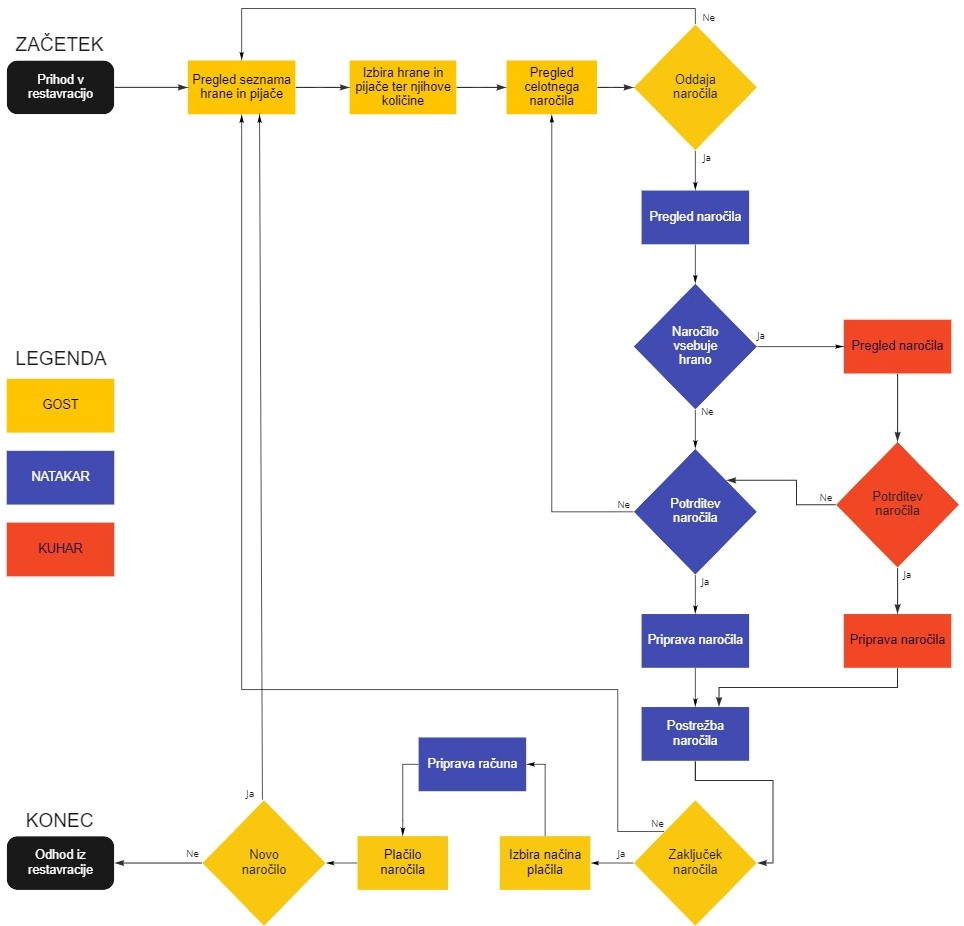
\includegraphics[width=13cm]{Diagram_poteka.jpg}
\caption{Postopek izvedbe in zaključka elektronskega naročila v restavraciji}
\label{Diagram1}
\end{figure}

Gost s sprehajanjem skozi menije izbira hrano in pijačo ter jo sproti dodaja v naročilo (slika~\ref{Opis1}).
V našem primeru gost izbere dva sokova in dve pici. Pregled naročila izvede v košarici, kjer naročilo tudi odda (sliki~\ref{Opis2} in~\ref{Opis22}). Natakar in kuhar se najprej prijavita, da se omogoči pregled naročil. Na seznamu se jima prikaže novo naročilo, pri čemer morata preveriti, ali imata vse sestavine za pripravo (sliki~\ref{Opis3} in~\ref{Opis33}). V našem primeru naročilo vsebuje hrano, tako da mora naročilo najprej potrditi kuhar (sliki~\ref{Opis4} in~\ref{Opis44}), da lahko natakar celotno naročilo potrdi gostu (sliki~\ref{Opis5} in~\ref{Opis55}). Ko je hrana pripravljena, kuhar o tem obvesti natakarja. Natakar naročilo postreže in naročilo označi kot postreženo. Gost zaključi naročilo z zahtevanjem račun v zavihku košarica, kjer je naročilo tudi oddal. Način plačila izbere ob kliku na zahtevo (slika~\ref{Opis6}). Natakar je obveščen o zahtevi za račun in načinu plačila gosta (slika~\ref{Opis66}). S tiskanjem računa natakar zaključi naročilo, s čimer se to izbriše s seznama aktivnih naročil.
\begin{figure}[!htb]
\centering
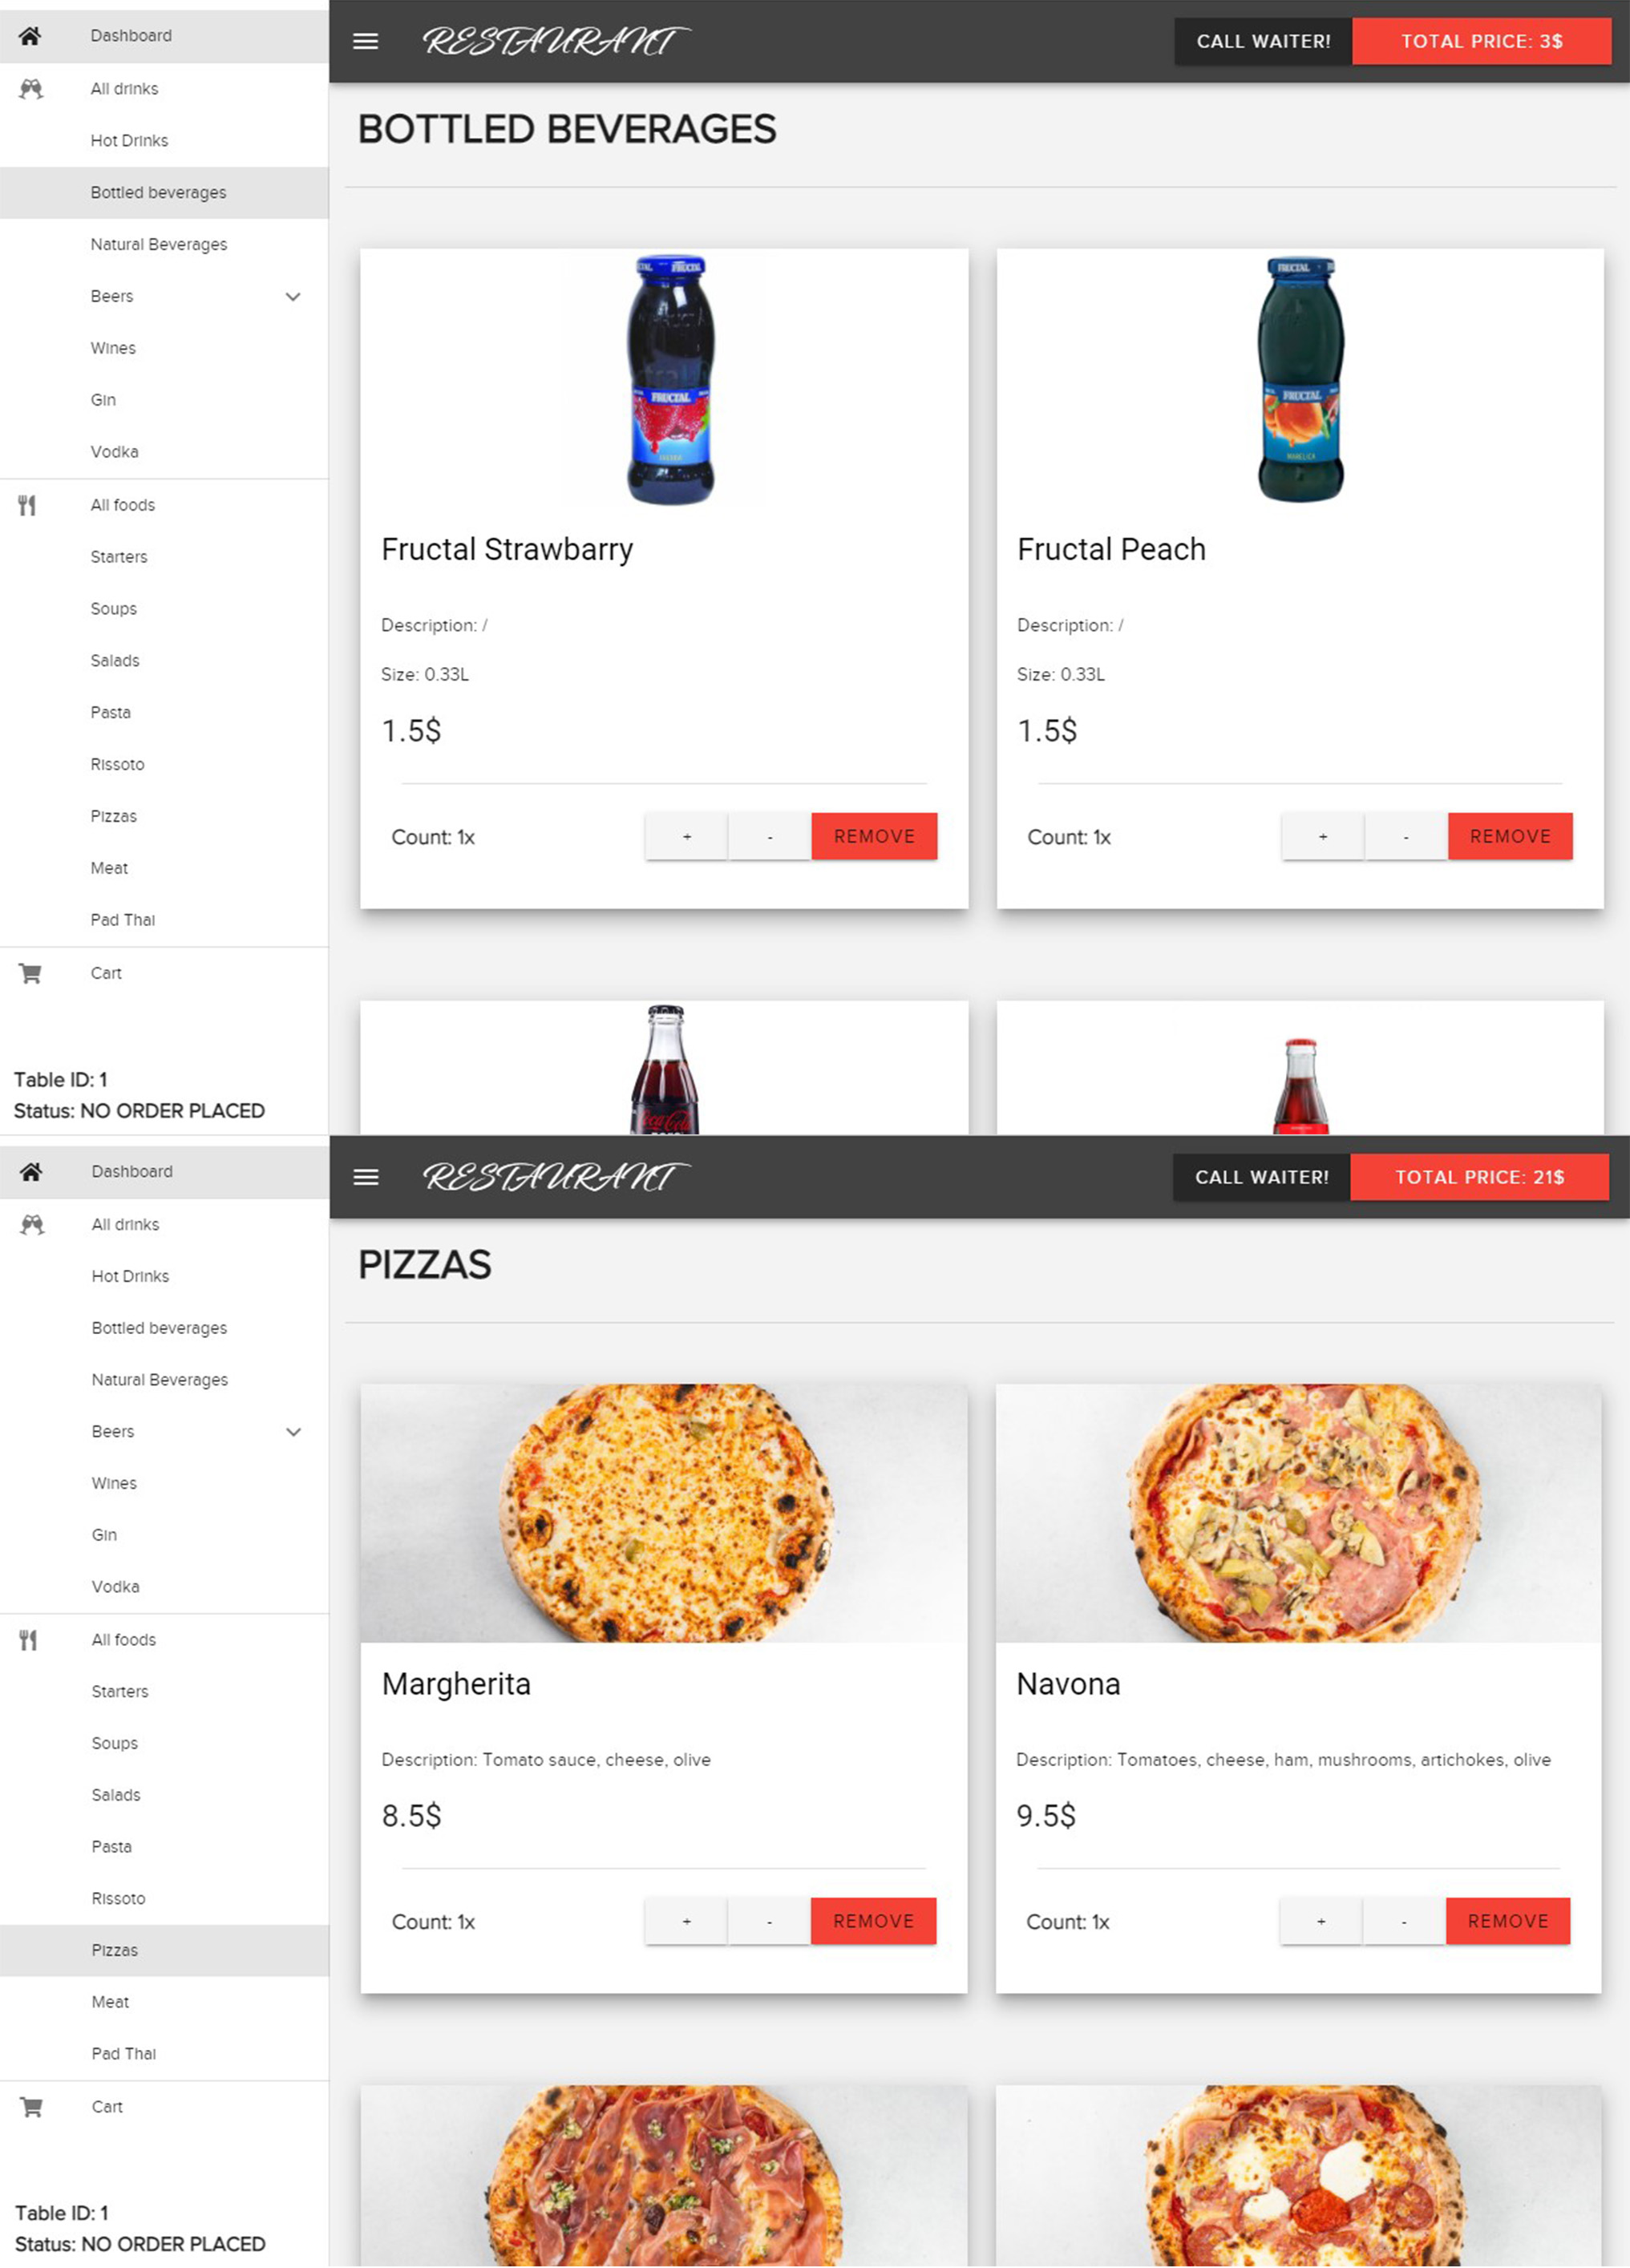
\includegraphics[width=10cm]{narocanje.jpg}
\caption{Pregled in izbiranje hrane in pijače}
\label{Opis1}
\end{figure}

\begin{figure}
\centering
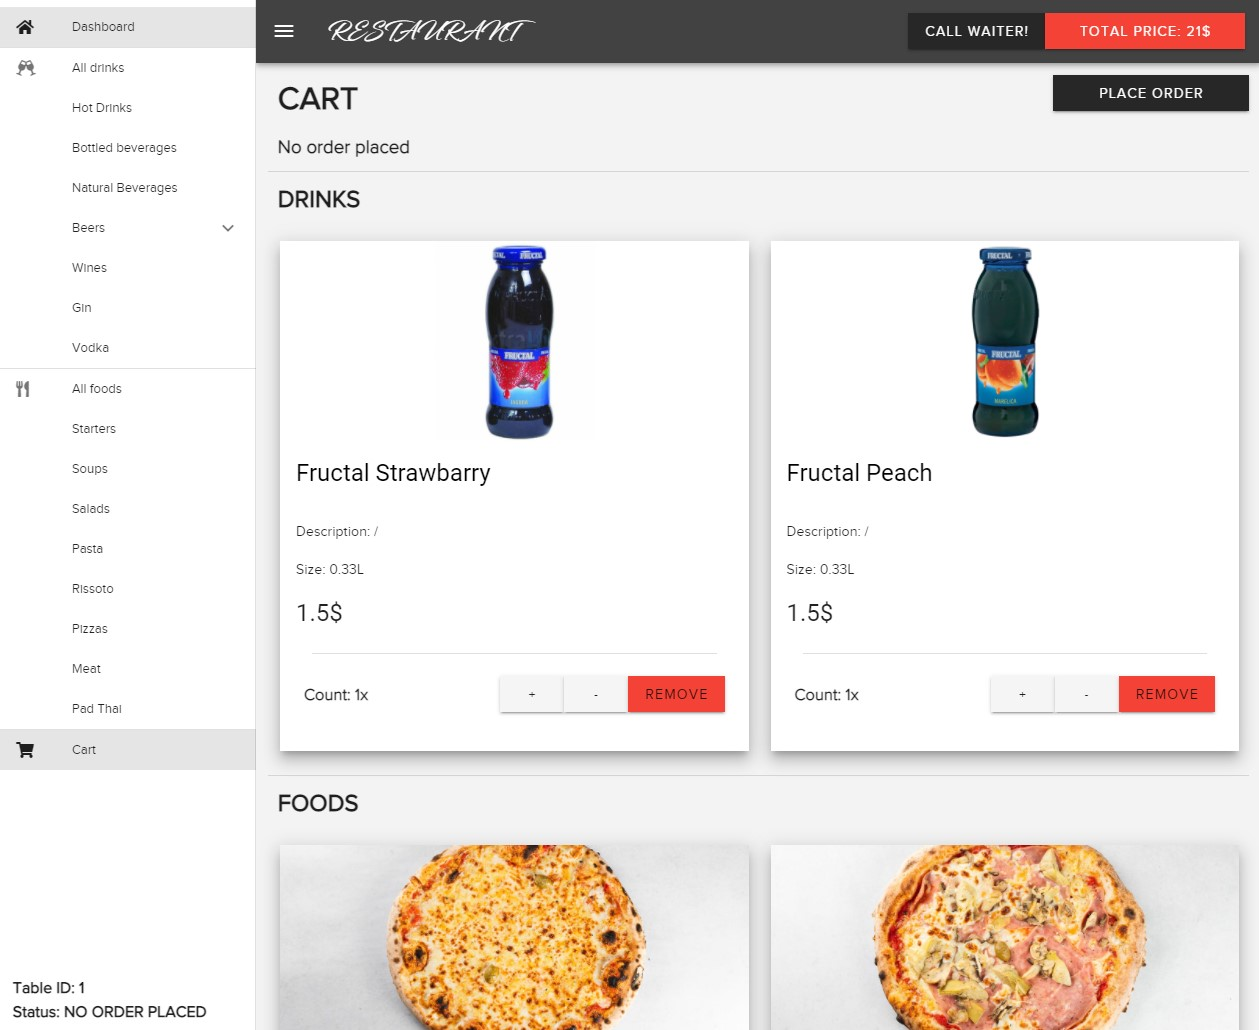
\includegraphics[width=11cm]{order_2.jpg}
\caption{Pregled košarice}
\label{Opis2}
\end{figure}
\begin{figure}
\centering
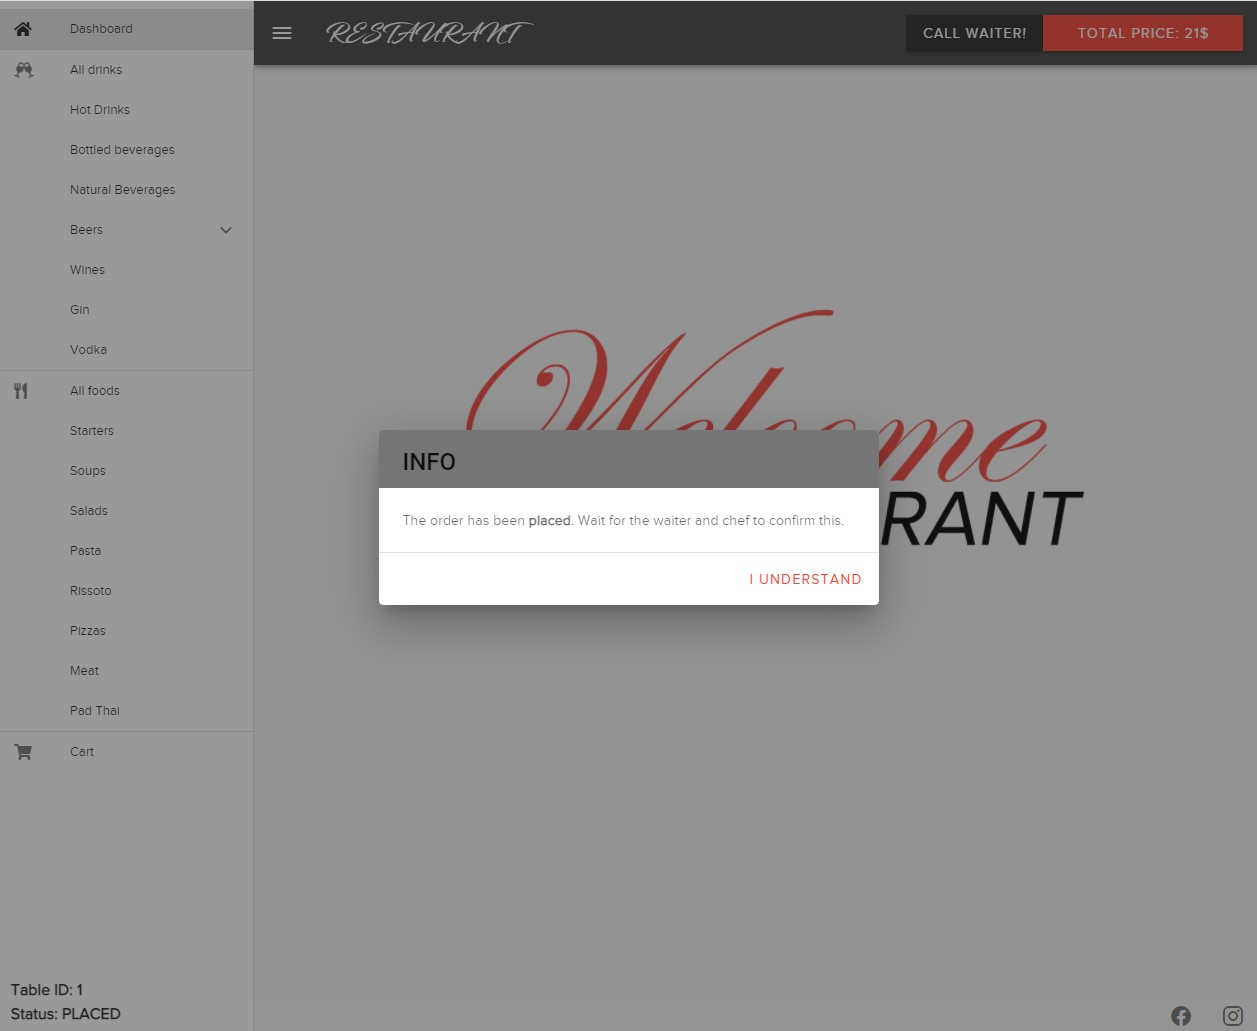
\includegraphics[width=11cm]{order_3.jpg}
\caption{Oddajanje naročila}
\label{Opis22}
\end{figure}

\begin{figure}
\centering
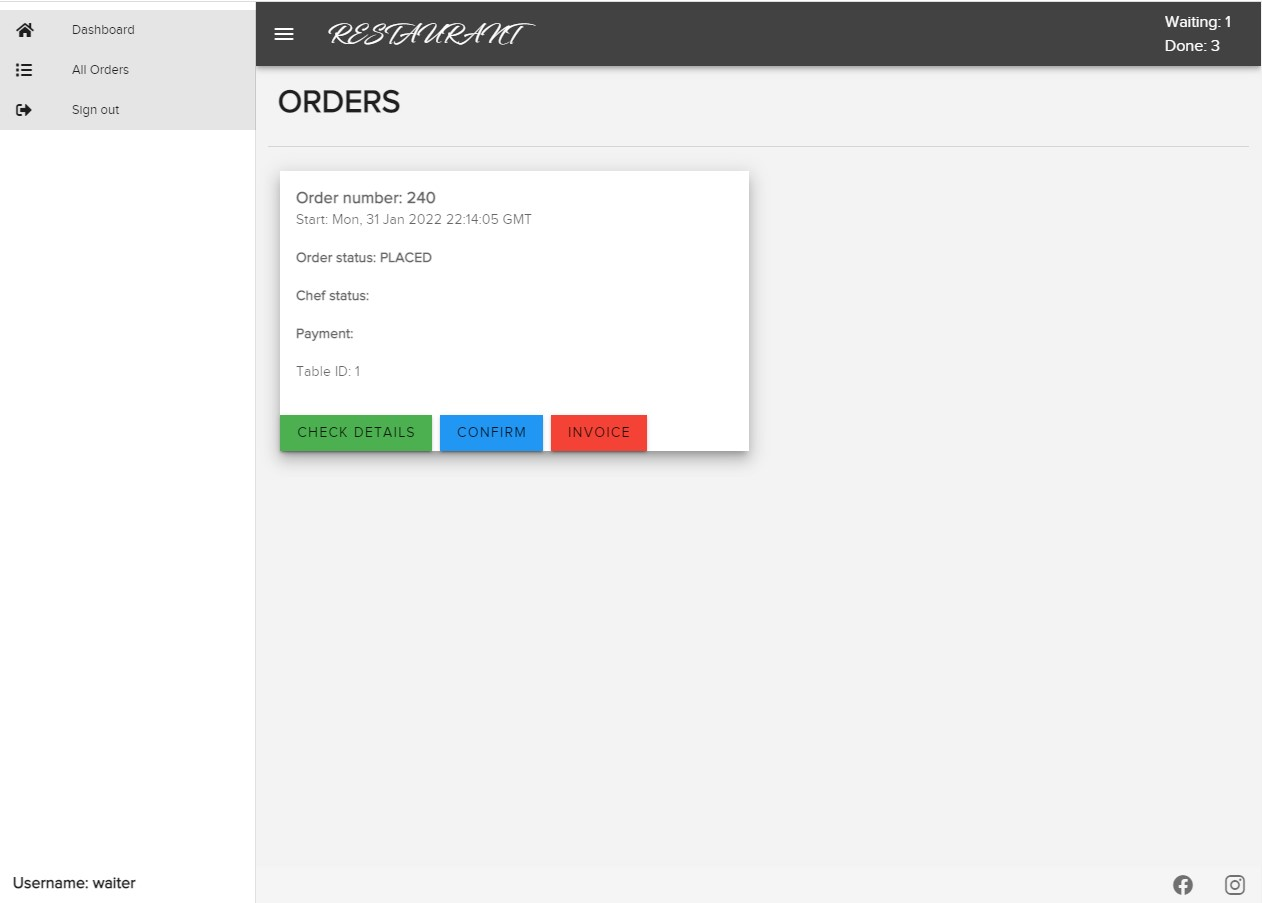
\includegraphics[width=12cm]{order_4.jpg}
\caption{Pregled naročila, kot ga vidi natakar}
\label{Opis3}
\end{figure}
\begin{figure}
\centering
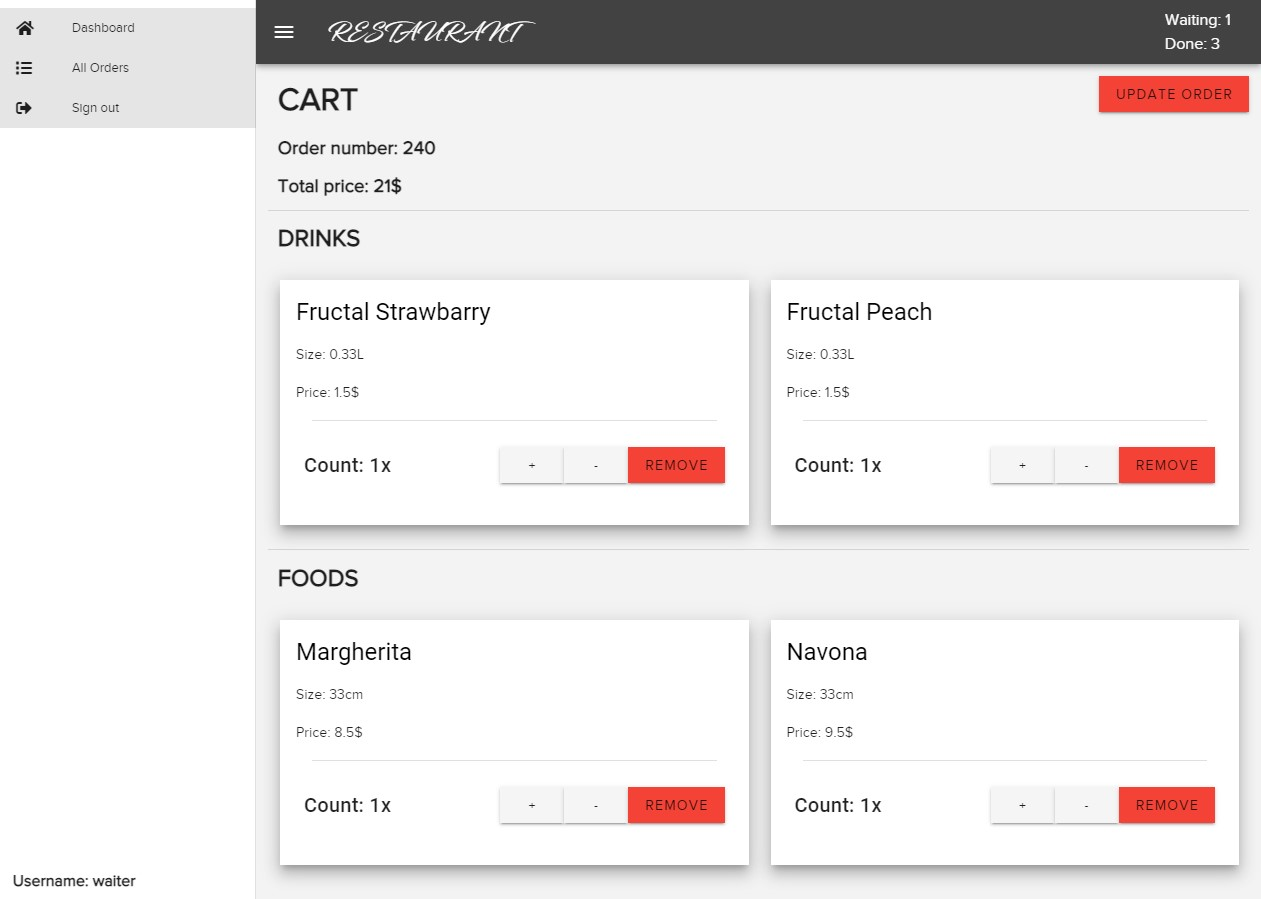
\includegraphics[width=12cm]{order_5.jpg}
\caption{Pregled podrobnosti naročila, kot ga vidi natakar}
\label{Opis33}
\end{figure}


\begin{figure}
\centering
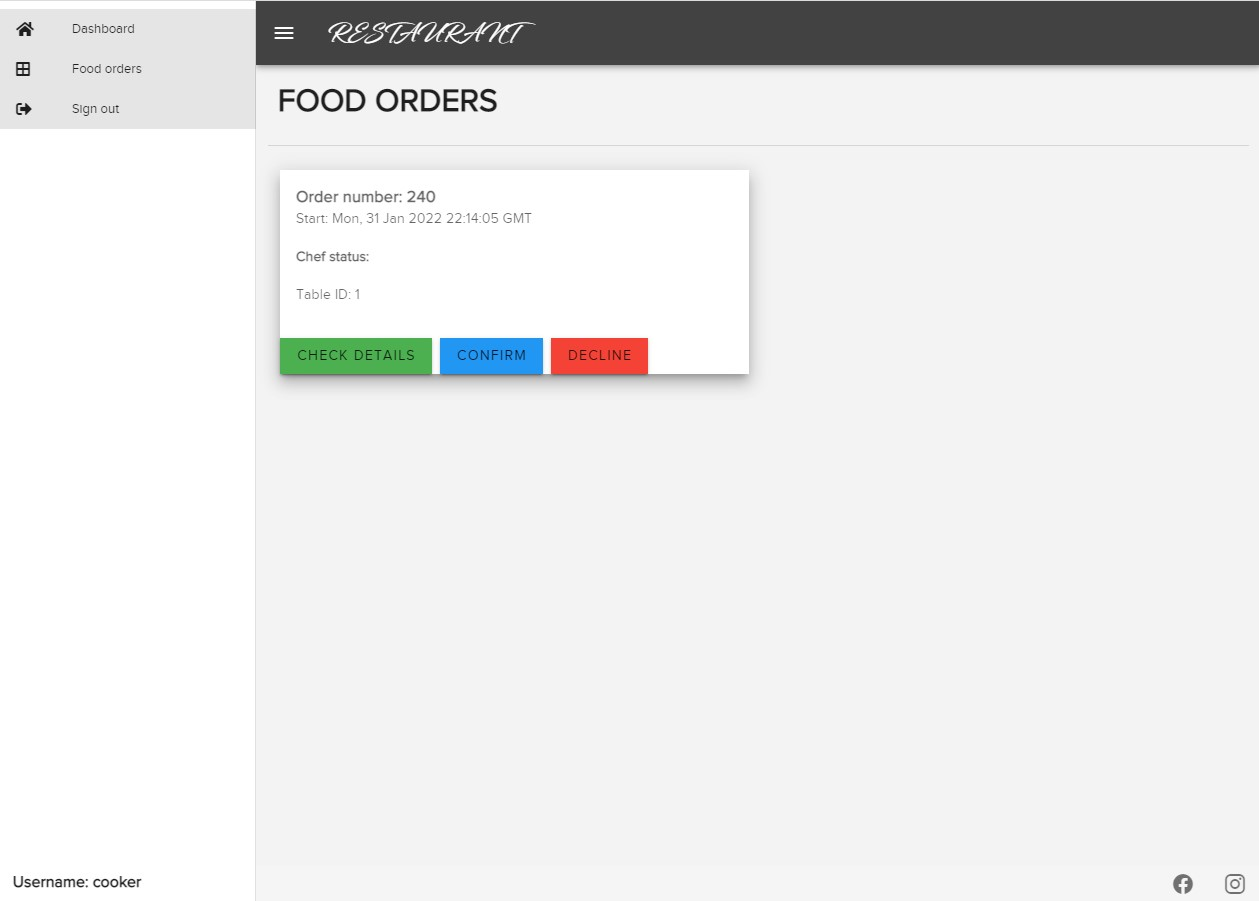
\includegraphics[width=12cm]{order_6.jpg}
\caption{Pregled naročila, kot ga vidi kuhar}
\label{Opis4}
\end{figure}
\begin{figure}
\centering
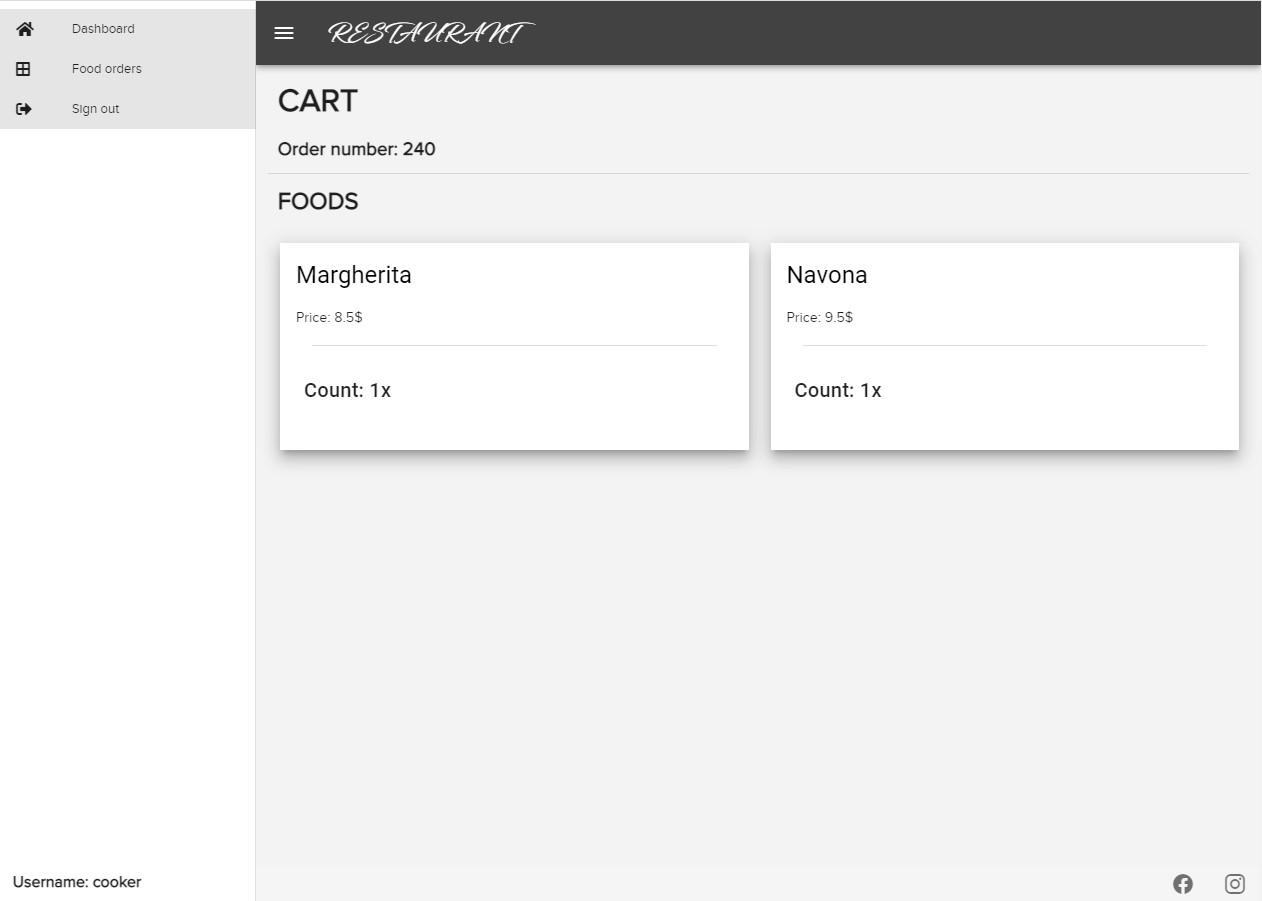
\includegraphics[width=12cm]{order_7.jpg}
\caption{Pregled podrobnosti naročila, kot ga vidi kuhar}
\label{Opis44}
\end{figure}


\begin{figure}
\centering
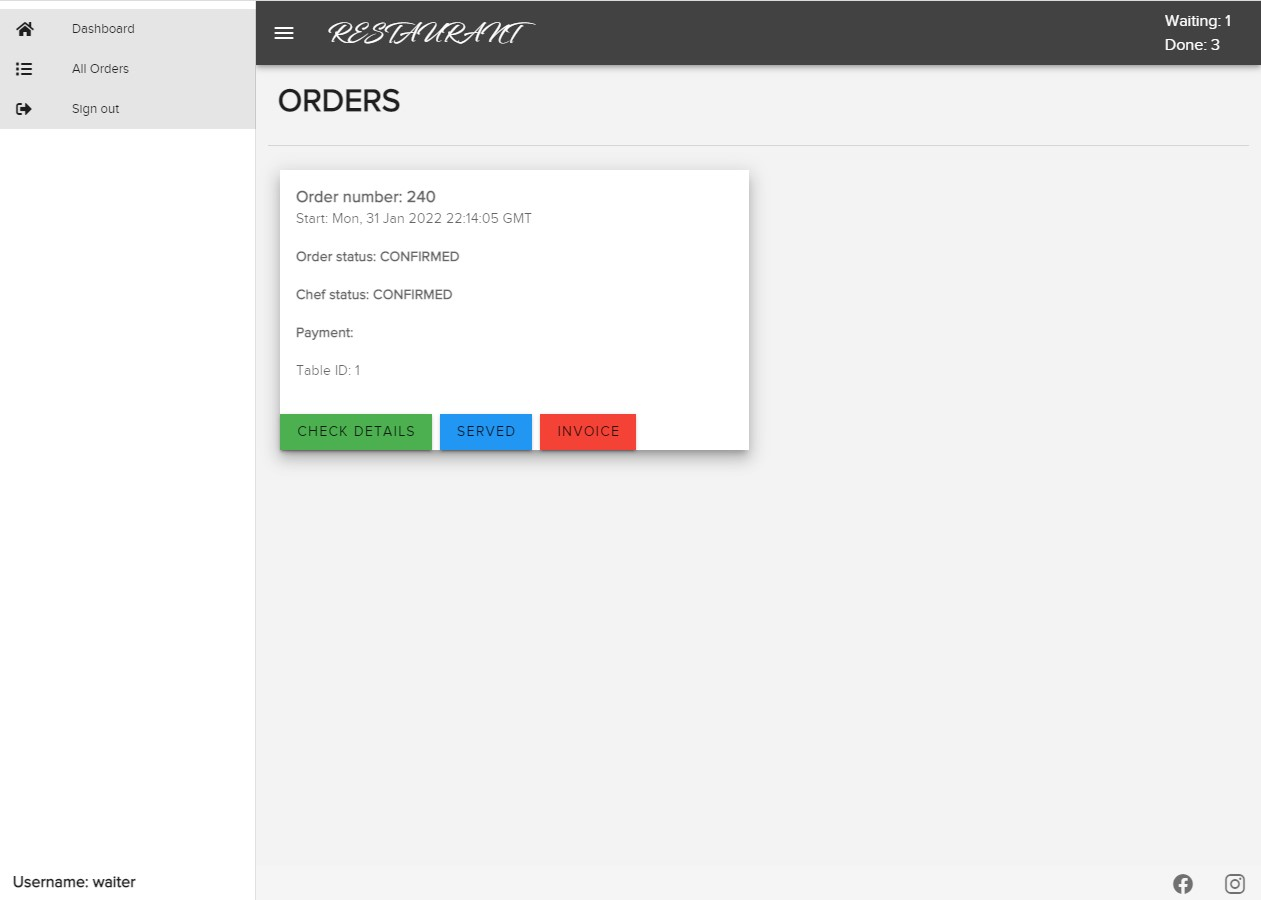
\includegraphics[width=11.5cm]{order_8.jpg}
\caption{Potrjevanje naročila}
\label{Opis5}
\end{figure}
\begin{figure}
\centering
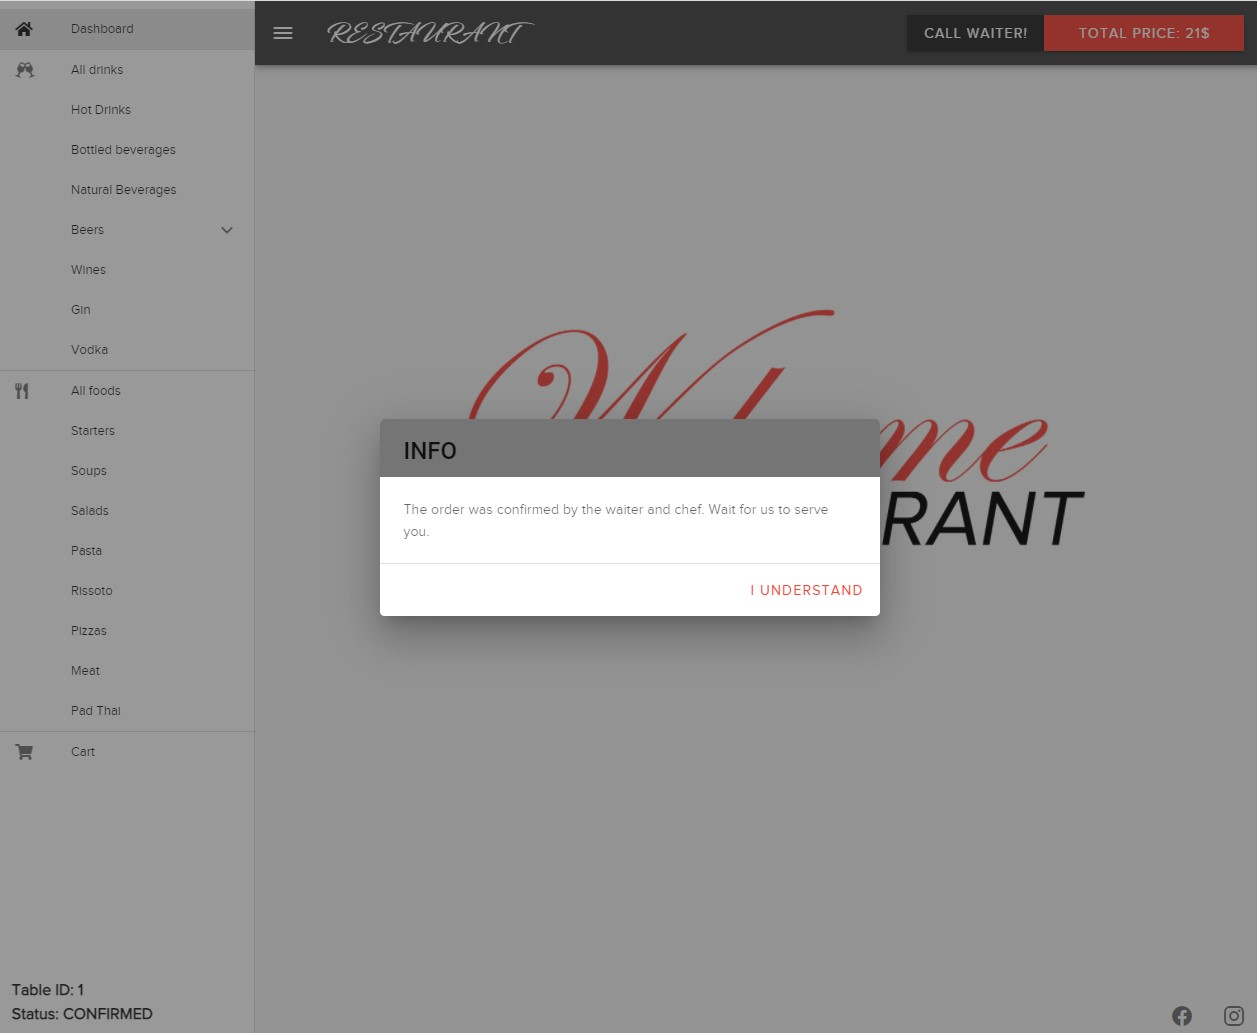
\includegraphics[width=11.5cm]{order_9.jpg}
\caption{Obveščanje gosta o sprejemu naročila}
\label{Opis55}
\end{figure}


\begin{figure}
\centering
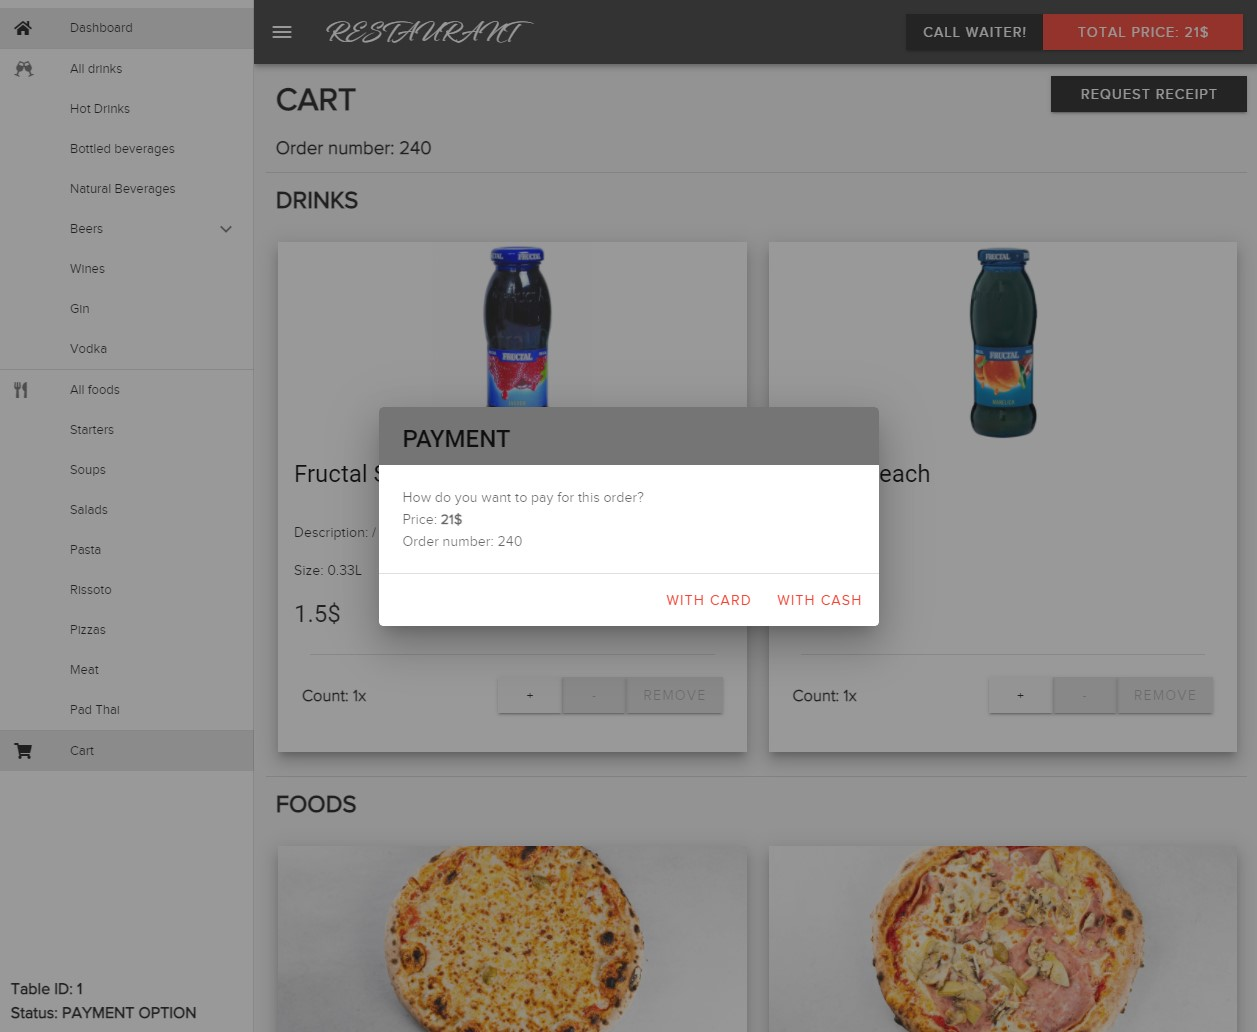
\includegraphics[width=11.5cm]{order_10.jpg}
\caption{Zahtevanje računa in izbira načina plačila}
\label{Opis6}
\end{figure}
\begin{figure}
\centering
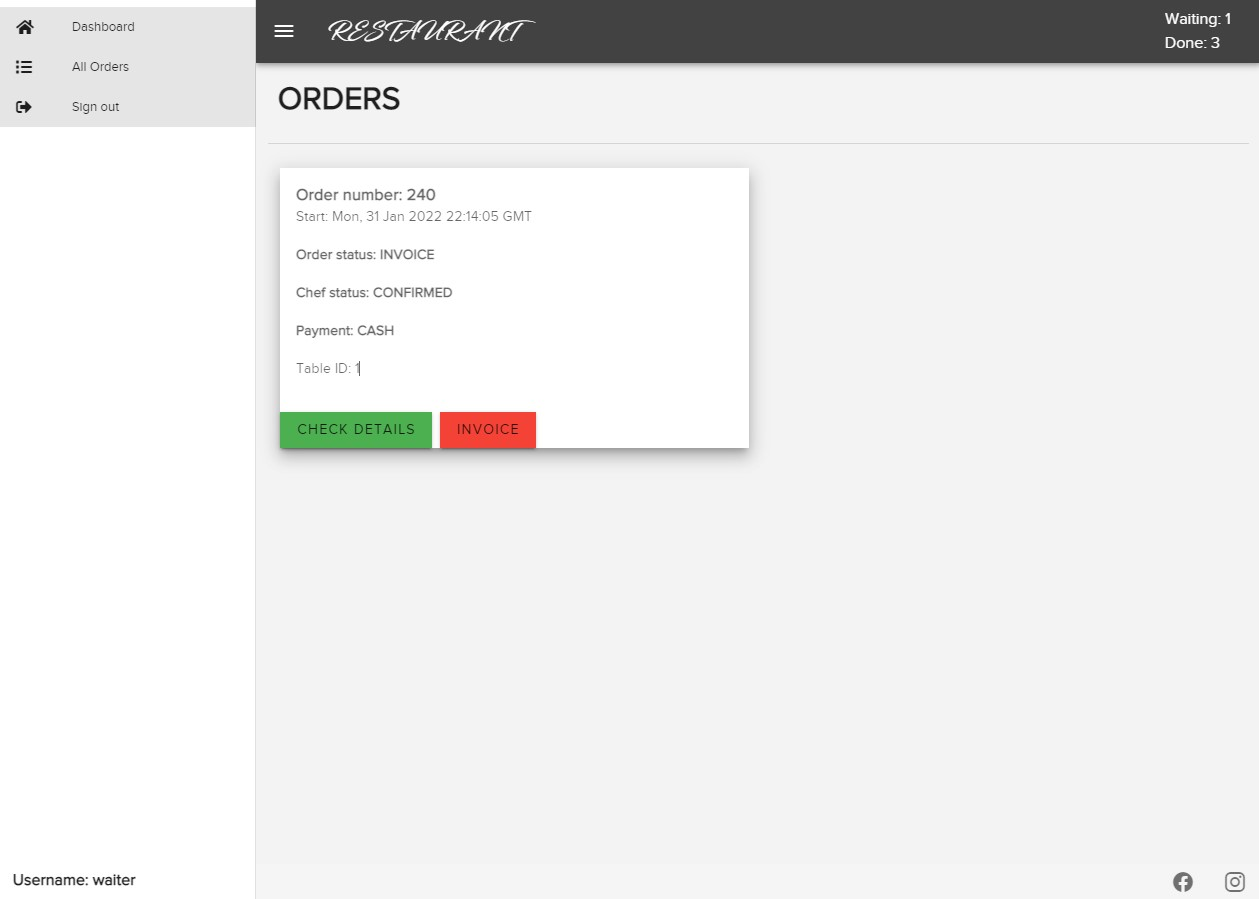
\includegraphics[width=11.5cm]{order_11.jpg}
\caption{Zaključevanje naročila s tiskanjem računa}
\label{Opis66}
\end{figure}


\clearpage
\section{Implementirana rešitev}
Trenutna rešitev omogoča implementacijo le znotraj ene restavracije. Aplikacija bi bila nameščena na lokalnem spletnem strežniku. Naročanje bi gost izvajal s pomočjo tablic, ki bi bile nameščene na vsaki mizi v restavraciji. 

Nadgradnja bi predstavljala uporabo aplikacije za naročanje z branjem kode QR (angl. Quick Response), ki bi bila nameščena na vsaki mizi v restavraciji. V kodi bi bila zapisana ime restavracije in številka mize. Kodo bi gost skeniral z mobilno napravo s preusmeritvijo v aplikacijo. Celoten sistem bi deloval v odprtem internetnem omrežju, tako za goste kot tudi natakarje in kuharje. Strežnik bi lahko implementirali za eno ali večje število restavracij in bi omogočal storitev vsem restavracijam po Sloveniji. Treba bi bilo zagotoviti, da ne bi prihajalo do fantomskih naročil, kjer bi nepridipravi oddajali neveljavna naročila. Temu bi se lahko izognili na dva načina. Prvi način bi bil, da bi moral biti uporabnik prijavljen preko lokalnega omrežja, s čimer bi overil svojo dejansko prisotnost v restavraciji.
Drugi način bi bilo geslo, ki bi ga uporabnik prejel od natakarja. 


\section{Izboljšave}

Potrebne izboljšave, da bi lahko aplikacijo ponudili potencialnim kupcem, so:

1.) Možnost, da lahko vsak posameznik za mizo dodaja hrano in pijačo k naročilu.

2.) Možnost hkratnega delovanja več kuharjev, kot smo to implementirali za natakarje.

3.) Administrativni dostop za urejanje menijev.

4.) Spremljanje zaloge hrane in pijače.

5.) Dodatno spremljanje hrane in pijače za kuharja/natakarja, kot npr. katera pijača in hrana je že bila postrežena.


Napredne izboljšave: 

1.) Statistika za lastnika restavracije, ki bi poleg vseh podatkov izračunala predvideno oceno nabave za prihodnji mesec.

2.) Neposredno brezstično plačevanje s plačilno kartico za gosta.

3.) Če bi aplikacija delovala v odprtem internetnem omrežju, bi lahko restavracije oglaševale dostavo ali sprejemale naročila za dostavo hrane in pijače.


\chapter {Sklepne ugotovitve}
Namen diplomske naloge je bil izdelati enostavno aplikacijo, ki bi olajšala delo natakarjem in nudila kakovostnejšo postrežbo gostom. Mislimo, da je aplikacija v okviru diplomskega dela realizirana v skladu z zahtevami, pričakovanji in cilji. Uporaba aplikacije gostom ponuja drugačno uporabniško izkušnjo, ki omogoča tudi klasično izbiro naročanja z neposrednim stikom z natakarjem. S tem smo želeli poudariti, da aplikacija ni namenjena nadomestitvi delovnih mest natakarjev, vendar omogoča digitalizacijo procesov pri izvajanju njihovega dela. Natakarjeva glavna naloga bi še vedno bila postrežba gosta in priprava pijače. 

Aplikacija bi bila s predstavljenimi izboljšavami primerna prototipna rešitev za uporabo. Uporabljali bi jo lahko v vsaki restavraciji, če ne drugače kot pomoč ob veliki zasedenosti. Trenutno, v času krize, povezane z epidemijo covida-19, bi takšna aplikacija omogočala določeno podporo za delovanje restavracij tudi pri spletnem naročanju.


\newpage %dodaj po potrebi, da bo številka strani za Literaturo v Kazalu pravilna!
\ \\
\clearpage
\addcontentsline{toc}{chapter}{Literatura}
\bibliographystyle{plain}
\bibliography{literatura}


\end{document}

